%-*- coding:utf-8 -*-

\documentclass[10pt,dvipdfmx]{beamer}
\usepackage{tutorial}

\title{計算機実験II (L1) --- モンテカルロ法}
\date{2020/9/25}

\begin{document}

\begin{frame}
  \titlepage
  \tableofcontents
\end{frame}

\section{講義・実習の概要}

\begin{frame}[t]{講義・実習の目的}
  \begin{itemize}
    %\setlength{\itemsep}{1em}
  \item 理論・実験を問わず、学部〜大学院〜で必要となる現代的かつ普遍的な計算機の素養を身につける
  \item {\color{gray}UNIX環境に慣れる(シェル、ファイル操作、エディタ)}
  \item {\color{gray}ネットワークの活用 (リモートログイン、共同作業)}
  \item {\color{gray}プログラムの作成(C言語、コンパイラ、プログラム実行)}
  \item 基本的な数値計算アルゴリズム・数値計算の常識を学ぶ
  \item {\color{gray}科学技術文書作成に慣れる(\LaTeX, グラフ作成)}
  \item {\color{red}物理学における具体的な問題を通して実践的な知識と経験を身につける}
  \end{itemize}
\end{frame}

\begin{frame}[t]{身に付けて欲しいこと}
  \begin{itemize}
    %\setlength{\itemsep}{1em}
  \item ツールとしてないものは自分で作る (物理の伝統)
  \item すでにあるものは積極的に再利用する (車輪の再発明をしない)
  \item 数学公式と数値計算アルゴリズムは別物
  \item 刻み幅・近似度合いを変えて何度か計算を行う
  \item グラフ化して目で見てみる
  \item 計算量(コスト)のスケーリング(次数)に気をつける
  \item 記録に残す・再現性を確保する
  \item {\color{red}問題の解き方は一通りではない}
  \end{itemize}
\end{frame}

\begin{frame}[t]{講義・実習内容}
  \begin{itemize}
    \setlength{\itemsep}{1em}
  \item 問題解決型: 計算機実験Iで身に付けた知識をもとに、より高度な数値計算手法・アルゴリズムを学び、物理学における具体的な問題への応用を通して実践的な知識と経験を身につける
    \begin{itemize}
    \item 数値対角化と量子力学
    \item モンテカルロ法・分子動力学と統計物理
    \item 最適化問題
    \end{itemize}
  \item スタッフ \href{mailto:computer@exa.phys.s.u-tokyo.ac.jp}{computer@exa.phys.s.u-tokyo.ac.jp}
    \begin{itemize}
    \item 講義: 藤堂
    \item 実習: 鈴木(元早野研)、斉藤(古澤研)
    \item 実習TA: 山本(藤堂研D1)、近藤(藤堂研M1)
    \end{itemize}
  \end{itemize}    
\end{frame}

\begin{frame}[t]{質問がある場合には、、、}
  \begin{enumerate}
    %\setlength{\itemsep}{1em}
  \item ITC-LMS の掲示板を見る
  \item ハンドブック、講義資料を確認
  \item まわりの人に質問してみる
  \item ネットで検索
  \item 計算機実験担当者(\href{mailto:computer@exa.phys.s.u-tokyo.ac.jp}{computer@exa.phys.s.u-tokyo.ac.jp}) に相談
  \end{enumerate}
  メールで質問するときに注意すべきこと
  \begin{itemize}
  \item (メールの)標題をきちんとつける、きちんと名乗る
  \item 実行環境を明示する
  \item 問題を再現する手順を明記する
  \item 関連するファイル(Cや \LaTeX のソースコード等)を添付する
  \item エラーメッセージを添付する
  \end{itemize}
\end{frame}

\section{環境整備}

\begin{frame}[t,fragile]{計算機実験に必要な環境整備}
  \begin{itemize}
    % \setlength{\itemsep}{1em}
  \item 「\href{https://github.com/utphys-comp/handbook/releases/download/handbook-2021/handbook.pdf}{計算機実験ハンドブック}」に書いてあることが、自分のPCで一通り試せるような環境を準備する
    \begin{itemize}
      % \setlength{\itemsep}{1em}
    \item プログラミング (オフライン・リモート利用)

      エディタ、コンパイラ(C, C++, Fortran, BLAS/LAPACK, MPI/OpenMP)
    \item 計算結果のプロット (オフライン利用)

      gnuplot (python/matplotlib, MATLAB でも可)
    \item 文書(レポート、論文)の作成 (オフライン・クラウド利用)

      \LaTeX (TeX Live あるいは Overleaf)
    \item ネットワークの利用 (ECCSなどの大学の計算機にリモートアクセスできる環境)

      ターミナル、SSH
    \item インタプリタ環境 (オフライン・クラウド利用)

      MATLAB、Python
    \end{itemize}
  \item 「\href{https://utphys-comp.github.io}{計算機実験のための環境整備}」({\small \href{https://utphys-comp.github.io}{https://utphys-comp.github.io}})を参考に、環境を整備する $\Rightarrow$ 実習1
  \end{itemize}
\end{frame}


%% \section{多体系の統計力学}

%% \begin{frame}[t,fragile]{典型的な統計力学モデル}
  \begin{itemize}
    %\setlength{\itemsep}{1em}
  \item 古典粒子系
    \begin{itemize}
    \item 調和振動子 \ \ $\displaystyle H = \frac{p^2}{2m} + \frac{k}{2}x^2$
    \item 多粒子系
      \[
      H = \sum \frac{p_i^2}{2m} + \sum_{ij} V(x_i, x_j)
      \]
    \item バネビーズ模型
      \[
      H = \sum \frac{p_i^2}{2m} + \frac{k}{2} \sum_{ij} (x_i-x_j)^2
      \]
  \end{itemize}
  \item 磁性体
    \begin{itemize}
    \item イジング模型 \ \ $\displaystyle H = -J \sum_{ij} \sigma_i \sigma_j$ \ \ \ $\sigma_i = \pm 1$
    \end{itemize}
  \end{itemize}
\end{frame}

%% %-*- coding:utf-8 -*-

\begin{frame}[t,fragile]{多体系の統計力学}
  \begin{itemize}
    %\setlength{\itemsep}{1em}
  \item カノニカル分布 \ $\pi(s) = \exp [- \beta H(s) ] / Z$ \ \ \ ($\beta = k_{\rm B} T$)
  \item 分配関数・自由エネルギー
    \begin{align*}
      Z(T) &= \int \exp [- \beta H(p,x) ] \, dp \, dx \qquad \text{(連続変数)} \\
      &= \sum_s \exp [- \beta H(s) ] \qquad \text{(離散変数)} \\
      f(T) &= - \beta^{-1} \log Z(T)
    \end{align*}
  \item 物理量の期待値
    \begin{align*}
      \langle A \rangle &= Z^{-1} \int A(p,x) \exp [- \beta H(p,x) ] \, dp \, dx \qquad \text{(連続変数)} \\
      &= Z^{-1} \sum_s A(s) \exp [- \beta H(s) ] \qquad \text{(離散変数)}
    \end{align*}
  \end{itemize}
\end{frame}

%% %-*- coding:utf-8 -*-

\begin{frame}[t,fragile]{多体系の統計力学}
  \begin{itemize}
    % \setlength{\itemsep}{1em}
  \item 内部エネルギー
    \begin{align*}
      E &= -\frac{\partial}{\partial\beta} \log Z = Z^{-1} \sum_s H(s) \exp [- \beta H(s) ] = \langle H \rangle
    \end{align*}
  \item 比熱
    \begin{align*}
      C &= \frac{1}{N} \frac{\partial E}{\partial T} = \frac{\beta^2}{N} (\langle H^2 \rangle - \langle H \rangle^2)
    \end{align*}
  \end{itemize}
\end{frame}

%% %-*- coding:utf-8 -*-

\begin{frame}[t,fragile]{様々な数値計算手法}
  \begin{itemize}
    % \setlength{\itemsep}{1em}
  \item 数え上げ (離散変数)
    \begin{itemize}
      \item 計算コスト × (指数関数的)
      \item メモリコスト ○ (${\cal O}(1)$)
    \end{itemize}
  \item 転送行列法 (離散変数)
    \begin{itemize}
      \item 計算コスト △ (指数関数的)
      \item メモリコスト △ (指数関数的)
    \end{itemize}
  \item 分子動力学法 (連続変数)
    \begin{itemize}
      \item 計算コスト ○ (${\cal O}(N)$)
      \item メモリコスト ○ (${\cal O}(N)$)
      \item 統計誤差あり
    \end{itemize}
  \item マルコフ連鎖モンテカルロ法 (離散変数・連続変数)
    \begin{itemize}
      \item 計算コスト ○ (${\cal O}(N)$)
      \item メモリコスト ○ (${\cal O}(N)$)
      \item 統計誤差あり
    \end{itemize}
  \end{itemize}
\end{frame}


\section{乱択アルゴリズム}
\begin{frame}[t,fragile]{乱択アルゴリズム(randomized algorithm)}
  \begin{itemize}
    %\setlength{\itemsep}{1em}
  \item 実行中に乱数を参照してその値によって振る舞いをかえるアルゴリズム
  \item ラスベガスアルゴリズム
    \begin{itemize}
    \item 乱数の出方によらず常に正しい結果を与えるアルゴリズム
    \item 平均化効果を利用するアルゴリズム:クイックソート
    \end{itemize}
  \item モンテカルロアルゴリズム
    \begin{itemize}
    \item 乱数の出方によっては誤った結果を与えるアルゴリズム
    \item 標本を利用するアルゴリズム:最大カット問題
    \item くじ引き型のアルゴリズム:素数性判定、関数の同一性、行列積の検算
    \item サンプリングアルゴリズム:モンテカルロ積分、マルコフ連鎖モンテカルロ
    \end{itemize}
  \end{itemize}
\end{frame}

\begin{frame}[t,fragile]{乱択クイックソート}
  \begin{itemize}
    %\setlength{\itemsep}{1em}
  \item 分割統治法に基づく再帰的なソートアルゴリズム
    \begin{itemize}
      \item 配列の中から要素を一つ選び、それより小さい要素からのみなる集合と大きい要素のみからなる集合の2つに分ける
      \item それぞれの集合をソートし、結合する
    \end{itemize}
    \item ほぼ同じ大きさの集合に分けることができる場合の実行ステップ数$\sim {\cal O}(n \log n)$
    \item 最悪(選んだ要素が常に最大 or 最小値)の場合のステップ数$\sim {\cal O}(n^2)$
    \item 分割に用いる要素を「ランダムに」選ぶ $\Rightarrow$ 平均ステップ数$\sim {\cal O}(n \log n)$
  \end{itemize}
\end{frame}

\begin{frame}[t,fragile]{クイックソート}
  \resizebox{!}{.7\textheight}{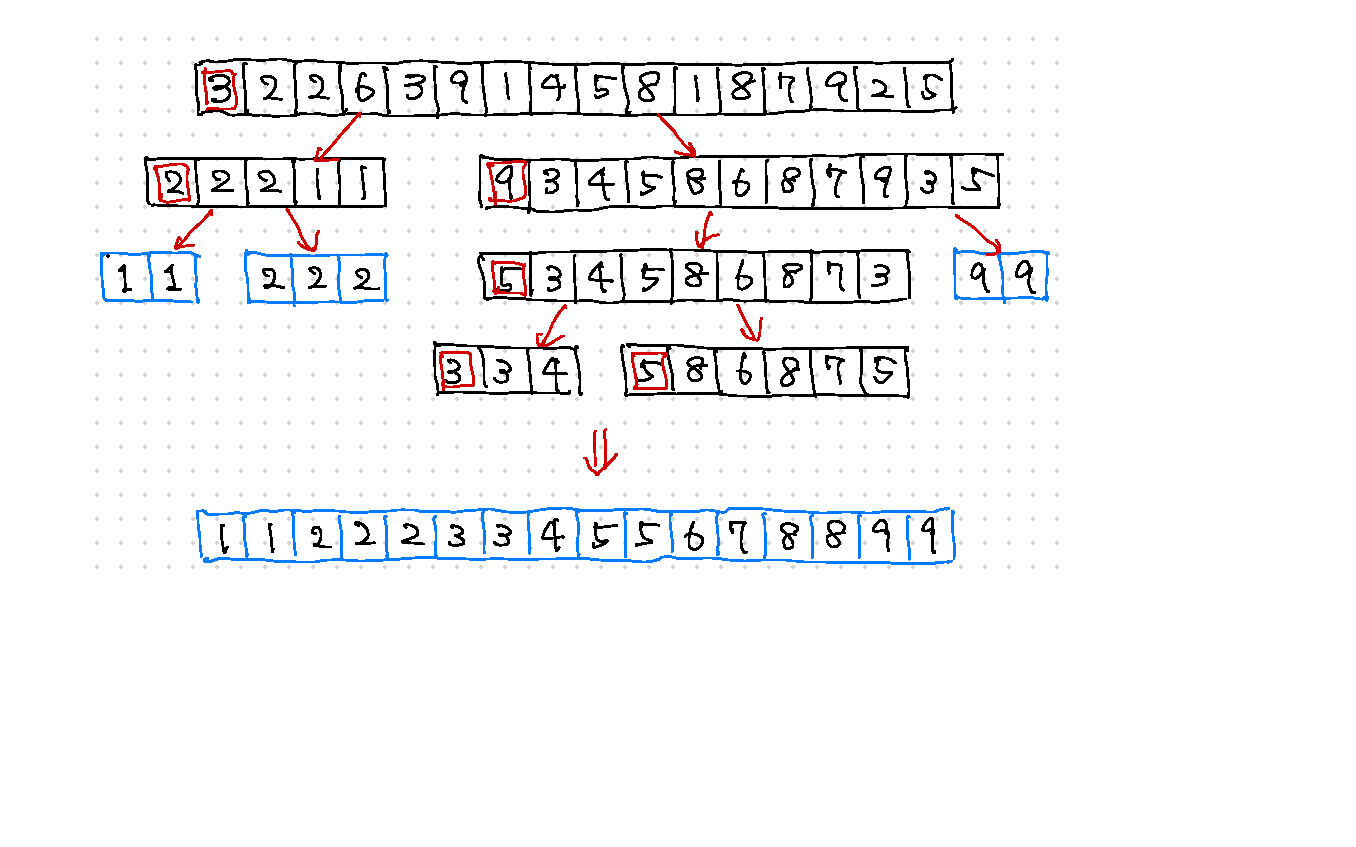
\includegraphics{image/quicksort.pdf}}
\end{frame}


\section{物理過程のシミュレーション}

\begin{frame}[t,fragile]{物質中の中性子輸送}
  \begin{center}
  \resizebox{0.45\textwidth}{!}{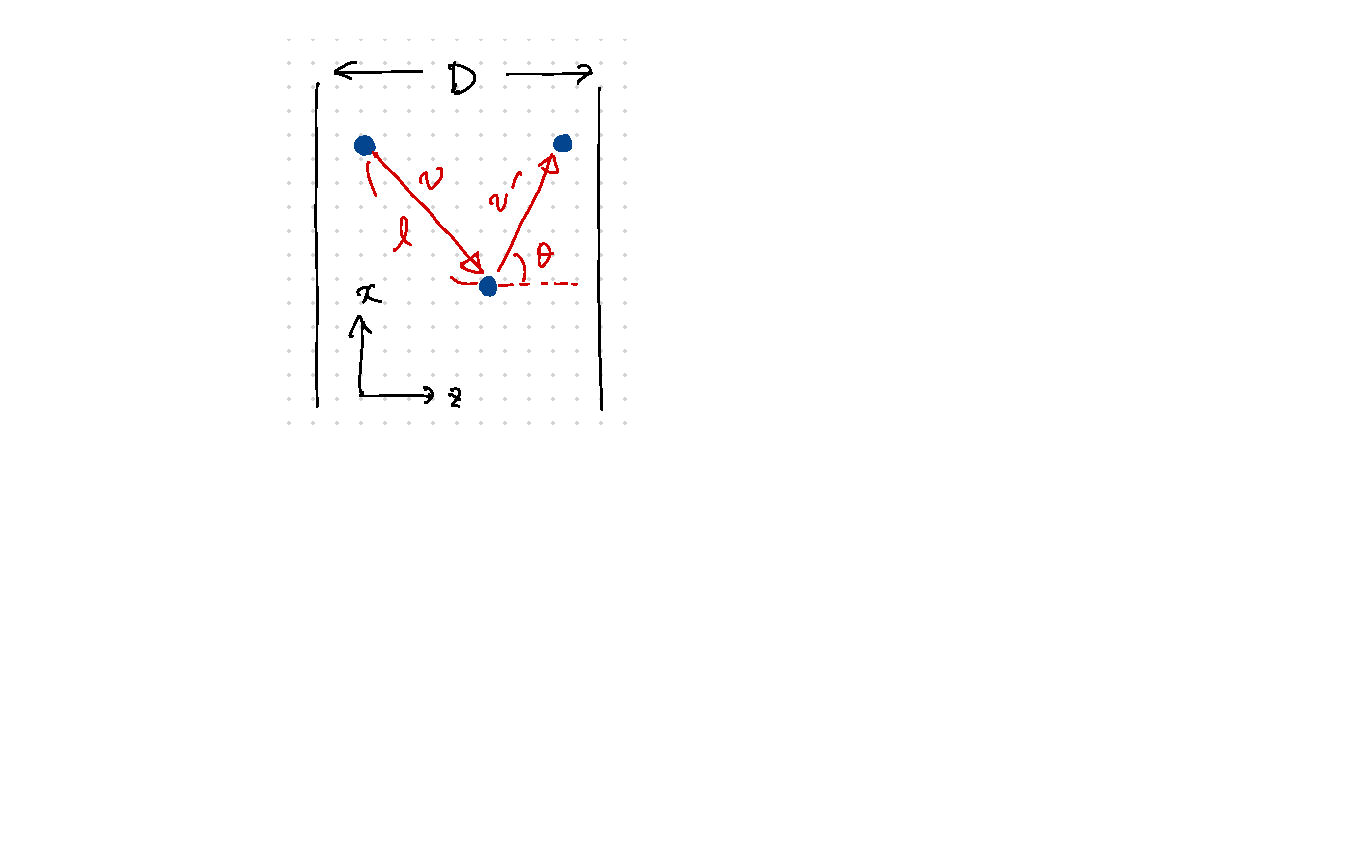
\includegraphics{image/scattering.pdf}}
  \end{center}
\end{frame}

\begin{frame}[t,fragile]{物質中の中性子輸送}
  \begin{itemize}
    %\setlength{\itemsep}{1em}
  \item ある板状の物質(厚さ$D$)に垂直に中性子が入射したときの吸収率・透過率・反射率
  \item 中性子はある確率で物質の原子核に衝突し、確率$p_{\rm c}$で吸収、$p_{\rm s}=1-p_{\rm c}$で散乱される
    \begin{itemize}
    \item 衝突は確率的に起きるので、次の衝突までの距離$\ell$は指数分布にしたがう($\lambda^{-1}$: 平均自由行程)
      \[
      p(\ell) = \lambda e^{-\lambda\ell}
      \]
    \item 衝突時、ランダムな方向に散乱されるとすると
      \[
      p(\theta,\phi) \, d\theta \, d\phi = \frac{d\Omega}{4\pi} = \frac{\sin \theta}{4\pi} \, d\theta \, d\phi
      \]
      \[
      p(\theta) = \frac{\sin \theta}{2} \qquad p(\phi)=\frac{1}{2\pi}
      \]
    \end{itemize}
  \end{itemize}
\end{frame}

\begin{frame}[t,fragile]{モンテカルロシミュレーション}
  \begin{enumerate}
    %\setlength{\itemsep}{1em}
  \item 初期条件 $z=0$, $\theta = 0$
  \item {\color{red} 指数分布から$\ell$を選ぶ}
  \item $z \leftarrow z + \ell \cos \theta$
  \item $z<0$ → 反射(終了) \\
    $z>D$ → 透過(終了) \\
    $0 < z < D$ → 確率$p_{\rm c}$で吸収(終了)、$p_{\rm s}$で散乱
  \item {\color{red} 散乱後の$\theta$を選び}、2に戻る
  \end{enumerate}
  \vspace*{-3.5cm}\hspace{8cm}\resizebox{0.25\textwidth}{!}{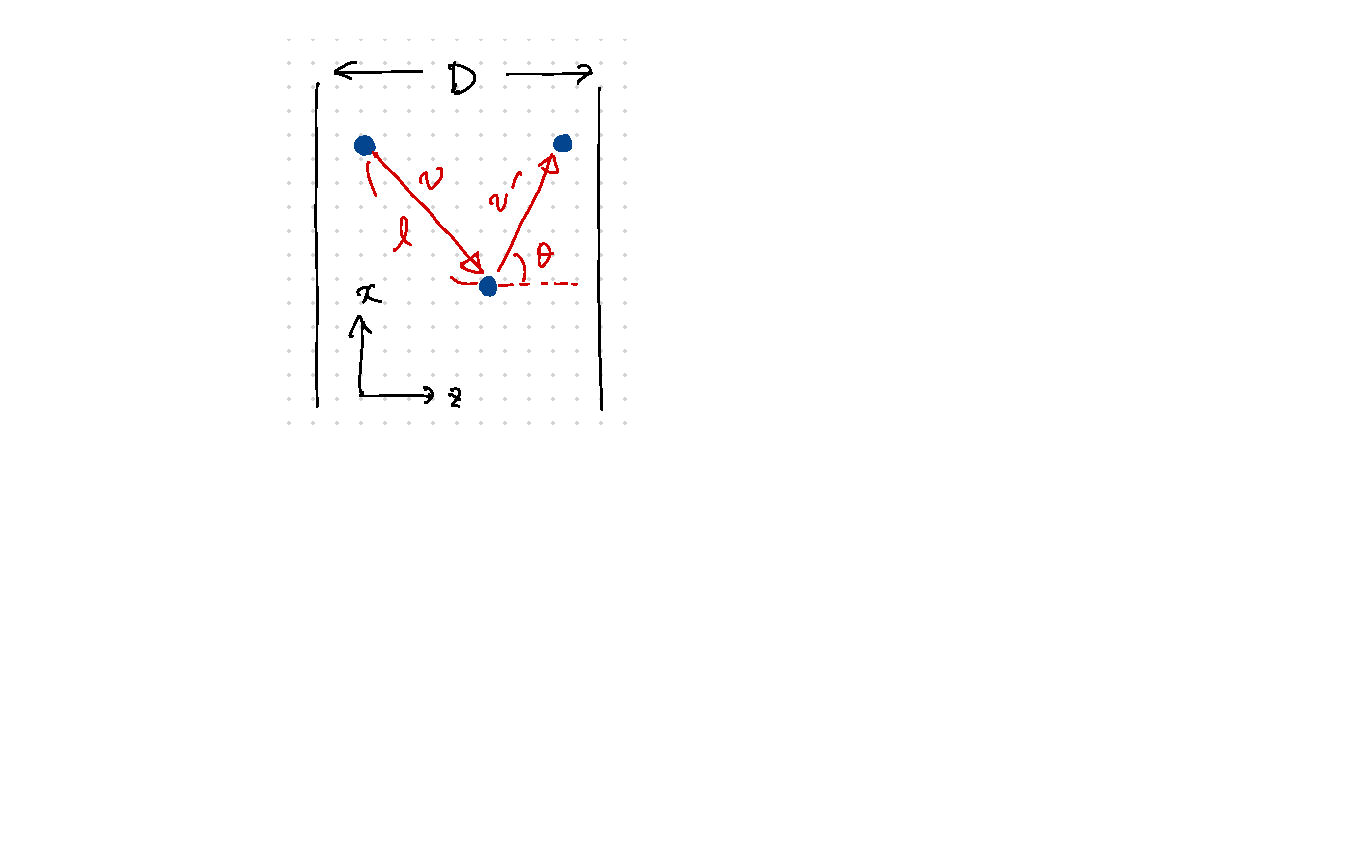
\includegraphics{image/scattering.pdf}}
\end{frame}



%\section{擬似乱数}

\begin{frame}[t,fragile]{乱数}
  \begin{itemize}
    \setlength{\itemsep}{1em}
  \item 自然乱数 (ハードウェア乱数)
    \begin{itemize}
    \item さいころ, コイン, ルーレット, 核分裂反応, 熱雑音, ショット雑音 ...
    \end{itemize}
  \item モンテカルロシミュレーションにおける必要条件
    \begin{itemize}
    \item 多数の乱数が必要
    \item ポータビリティ
    \item 生成速度
    \item 再現性
    \end{itemize}
  \item 擬似乱数 (pseudo random number)
    \begin{itemize}
    \item 計算機でプログラムに従って生成
    \item 分布の一様性, 相関, 周期に注意する必要あり
    \end{itemize}
  \end{itemize}
\end{frame}

\begin{frame}[t,fragile]{擬似乱数発生器}
  \begin{itemize}
    %\setlength{\itemsep}{1em}
  \item 最も簡単な乱数発生器:線形合同法 (linear congruential method)
    \[
    x_{n+1} = (ax_n+c) \ \mbox{mod} \ m
    \]
  \item 例) $a = 65539$, $c = 0$, $m = 2147483648$ (周期 $m-1$)
  \item 少しだけ異なる初期値 $(x0 = 1, 2, 3)$ から始めた場合
  \resizebox{!}{.35\textheight}{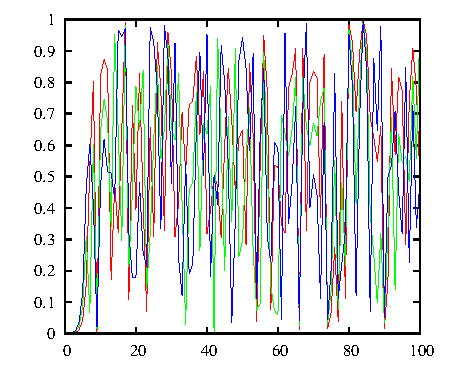
\includegraphics{image/lcg-1.pdf}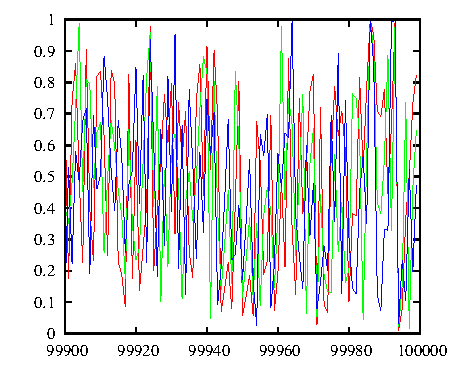
\includegraphics{image/lcg-2.pdf}}
  \item 数十ステップ進むとバラバラな振舞い ⇒ カオス的
  \end{itemize}
\end{frame}

\begin{frame}[t,fragile]{擬似乱数生成器における相関}
  \begin{itemize}
    %\setlength{\itemsep}{1em}
  \item 合同乗算法で多次元超立方体中に「ランダムに」点を打つと、それらの点は全て比較的小数の等間隔に並んだ超平面の上にのってしまう (多次元疎結晶構造)
  \resizebox{!}{.35\textheight}{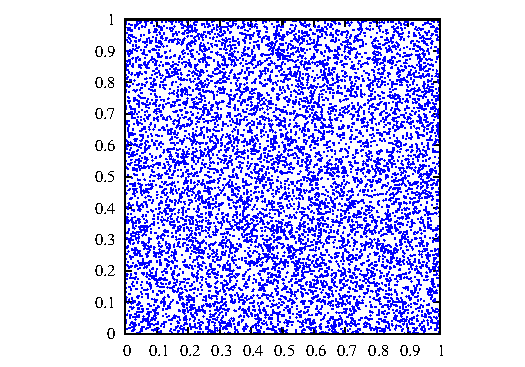
\includegraphics{image/lcg-2d.pdf}}
  \resizebox{!}{.35\textheight}{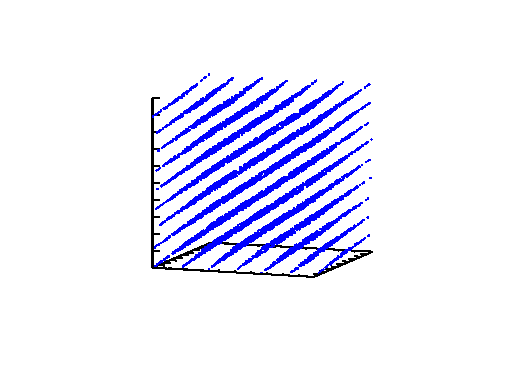
\includegraphics{image/lcg-3d.pdf}}
  \item 計算式に従って生成するため、必ず何らかの相関は残る
  \item できる限り相関が少なく周期の長い、理想的な乱数の開発が続けられている
    \begin{itemize}
    \item 現時点で、標準的な乱数発生器:メルセンヌ・ツイスター
    \item 周期 $2^{19937}-1$、高速、日本製! (例: \href{https://github.com/todo-group/computer-experiments/blob/master/exercise/monte_carlo/random.c}{example-2-L2/random.c})
    \end{itemize}
  \end{itemize}
\end{frame}

\begin{frame}[t,fragile]{乱数発生器の選び方}
  \begin{itemize}
    %\setlength{\itemsep}{1em}
  \item 万能乱数発生器は存在しない
  \item 生成された乱数のもつ性質について, 様々な数学的に厳密な証明, 多くのテスト結果がすでに存在するが, 特定のシミュレーションに使った場合の結果については何も保証してくれない
  \item 自分で乱数発生器を「発明」してはいけない
  \item 自分で乱数発生器をプログラムしてはいけない (既存のライブラリを使う)
  \item 初期化(種の設定)を正しく行う
  \item 実際にそれらしい乱数が生成されているか, 目でみて確認する
  \item 二種類以上の乱数発生器を使ってみて, 互いに一致する結果が出るかどうか確認する
  \end{itemize}
\end{frame}

\begin{frame}[t,fragile]{様々な分布}
  \begin{itemize}
    %\setlength{\itemsep}{1em}
  \item 乱数発生器は通常、一様な整数乱数あるいは実数乱数を生成
  \item 一様分布以外の分布にしたがう乱数の発生方法の代表例
  \item 逆関数法
    \begin{itemize}
      \item 確率分布関数$F(x)$の逆関数$F^{-1}(y)$ と(0,1)の一様乱数$u$から $v=F^{-1}(u)$
      \item 例: 指数分布 $p(x) = \frac{1}{\mu} e^{-x/\mu}$

      $F(x) = 1 - e^{-x/\mu}$ \ \ \ $F^{-1}(y) = - \mu \log(1-y)$
      \item 一般の確率分布関数について逆関数を求めるのは困難
    \end{itemize}
  \item 棄却法
    \begin{itemize}
      \item 確率密度関数を完全に囲むような箱を用意し、その箱の中で一様乱数を生成
      \item 確率密度関数の下側の点が生成されたら、その$x$座標を乱数として採用。上側の点の場合には再度生成
      \item もとの確率密度関数よりも箱が大きくなりすぎると非効率
    \end{itemize}
  \end{itemize}
\end{frame}

\section{擬似乱数}
\begin{frame}[t,fragile]{乱数}
  \begin{itemize}
    \setlength{\itemsep}{1em}
  \item 自然乱数 (ハードウェア乱数)
    \begin{itemize}
    \item さいころ, コイン, ルーレット, 核分裂反応, 熱雑音, ショット雑音 ...
    \end{itemize}
  \item モンテカルロシミュレーションにおける必要条件
    \begin{itemize}
    \item 多数の乱数が必要
    \item ポータビリティ
    \item 生成速度
    \item 再現性
    \end{itemize}
  \item 擬似乱数 (pseudo random number)
    \begin{itemize}
    \item 計算機でプログラムに従って生成
    \item 分布の一様性, 相関, 周期に注意する必要あり
    \end{itemize}
  \end{itemize}
\end{frame}

\begin{frame}[t,fragile]{擬似乱数発生器の例}
  \begin{itemize}
    %\setlength{\itemsep}{1em}
  \item 最も簡単な乱数発生器:線形合同法 (linear congruential method)
    \[
    x_{n+1} = (ax_n+c) \ \mbox{mod} \ m
    \]
  \item 例) $a = 65539$, $c = 0$, $m = 2147483648$ (周期 $m-1$)
  \item 少しだけ異なる初期値 $(x0 = 1, 2, 3)$ から始めた場合
  \resizebox{!}{.35\textheight}{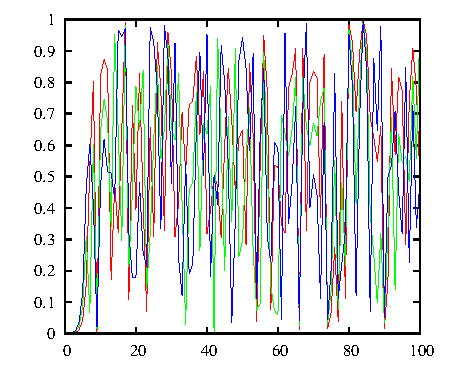
\includegraphics{image/lcg-1.pdf}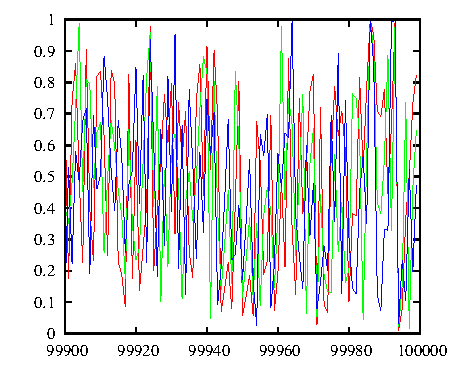
\includegraphics{image/lcg-2.pdf}}
  \item 数十ステップ進むとバラバラな振舞い ⇒ カオス的?
  \end{itemize}
\end{frame}

\begin{frame}[t,fragile]{擬似乱数生成器における相関}
  \begin{itemize}
    %\setlength{\itemsep}{1em}
  \item 合同乗算法で多次元超立方体中に「ランダムに」点を打つと、それらの点は全て比較的小数の等間隔に並んだ超平面の上にのってしまう (多次元疎結晶構造)
  \resizebox{!}{.35\textheight}{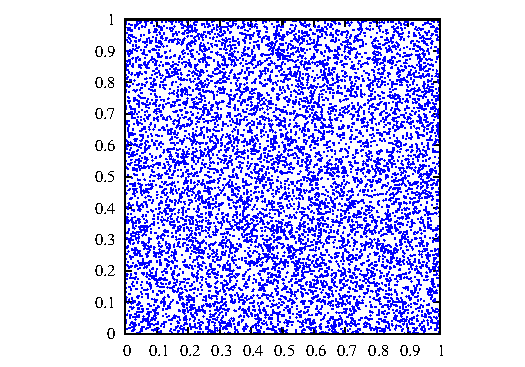
\includegraphics{image/lcg-2d.pdf}}
  \resizebox{!}{.35\textheight}{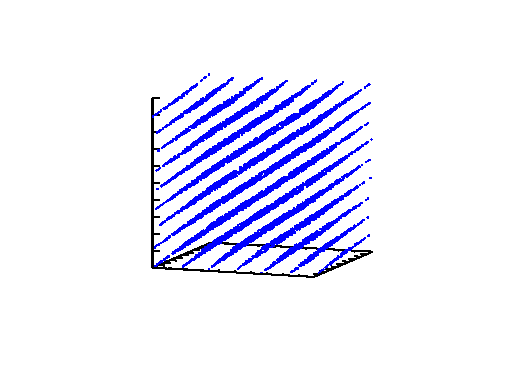
\includegraphics{image/lcg-3d.pdf}}
  \item 計算式に従って生成するため、必ず何らかの相関は残る
  \item できる限り相関が少なく周期の長い、理想的な乱数の開発が続けられている
    \begin{itemize}
    \item 現時点で、標準的な乱数発生器:メルセンヌ・ツイスター
    \item 周期 $2^{19937}-1$、高速、日本製! (例: \href{https://github.com/todo-group/computer-experiments/blob/master/exercise/monte_carlo/random.c}{random.c})
    \end{itemize}
  \end{itemize}
\end{frame}

\begin{frame}[t,fragile]{乱数発生器の選び方}
  \begin{itemize}
    %\setlength{\itemsep}{1em}
  \item 万能乱数発生器は存在しない
  \item 生成された乱数のもつ性質について, 様々な数学的に厳密な証明, 多くのテスト結果がすでに存在するが, 特定のシミュレーションに使った場合の結果については何も保証してくれない
  \item 自分で乱数発生器を「発明」してはいけない
  \item 自分で乱数発生器をプログラムしてはいけない (既存のライブラリを使う)
  \item 初期化(種の設定)を正しく行う
  \item 実際にそれらしい乱数が生成されているか, 目でみて確認する
  \item 二種類以上の乱数発生器を使ってみて, 互いに一致する結果が出るかどうか確認する
  \end{itemize}
\end{frame}

\begin{frame}[t,fragile]{様々な分布}
  \begin{itemize}
    %\setlength{\itemsep}{1em}
  \item 乱数発生器は通常、一様な整数乱数あるいは実数乱数を生成
  \item 一様分布以外の分布にしたがう乱数の発生方法の代表例
  \item 逆関数法
    \begin{itemize}
      \item 確率分布関数$F(x)$の逆関数$F^{-1}(y)$ と(0,1)の一様乱数$u$から $v=F^{-1}(u)$
      \item 例: 指数分布 $p(x) = \frac{1}{\mu} e^{-x/\mu}$

      $F(x) = 1 - e^{-x/\mu}$ \ \ \ $F^{-1}(y) = - \mu \log(1-y)$
      \item 一般の確率分布関数について逆関数を求めるのは困難
    \end{itemize}
  \item 棄却法
    \begin{itemize}
      \item 確率密度関数を完全に囲むような箱を用意し、その箱の中で一様乱数を生成
      \item 確率密度関数の下側の点が生成されたら、その$x$座標を乱数として採用。上側の点の場合には再度生成
      \item もとの確率密度関数よりも箱が大きくなりすぎると非効率
    \end{itemize}
  \end{itemize}
\end{frame}


% -*- coding: utf-8 -*-

\documentclass[10pt,dvipdfmx]{beamer}
\usepackage{tutorial}

\begin{document}
\section{ヒストグラム}
\begin{frame}[t,fragile]{疑似乱数とは}
  \begin{itemize}
    %\setlength{\itemsep}{1em}
  \item 計算機でプログラムに従って生成する乱数(のようなもの)
  \item 乱数は何に役立つか?
    \begin{itemize}
    \item 等式のチェック、例外の発見
    \item 初期値にランダムネスを入れることで最悪の場合を避ける
    \item サンプリングを使ったシミュレーション (→計算機実験II)
    \end{itemize}
  \item 乱数を使う場合の注意
    \begin{itemize}
    \item 計算式に従って生成するため周期は有限であり、必ず何らかの相関がある
    \item 初期化(種の設定)を正しく行う
    \item 実際にそれらしい乱数が生成されているか目で見て確認する
    \end{itemize}
  \item 代表的な乱数発生器のひとつ: メルセンヌ・ツイスター
    \begin{itemize}
    \item 周期 $2^{19937}-1$、高速、日本製!
    \item ヘッダファイル: \href{https://github.com/todo-group/computer-experiments/blob/master/exercise/monte_carlo/mersenne_twister.h}{mersenne\_twister.h}
    \item サンプルプログラム: \href{https://github.com/todo-group/computer-experiments/blob/master/exercise/monte_carlo/random.c}{random.c}
    \end{itemize}
  \end{itemize}
\end{frame}

\begin{frame}[t,fragile]{様々な分布}
  \begin{itemize}
    %\setlength{\itemsep}{1em}
  \item 乱数発生器は通常、一様な整数乱数あるいは実数乱数を生成
  \item 一様分布以外の分布にしたがう乱数の発生方法の代表例
  \item 逆関数法
    \begin{itemize}
      \item 確率分布関数$F(x)$の逆関数$F^{-1}(y)$ と(0,1)の一様乱数$u$から $v=F^{-1}(u)$
      \item 例: 指数分布 $p(x) = \frac{1}{\mu} e^{-x/\mu}$

      $F(x) = 1 - e^{-x/\mu}$ \ \ \ $F^{-1}(y) = - \mu \log(1-y)$
      \item 一般の確率分布関数について逆関数を求めるのは困難
    \end{itemize}
  \item 棄却法
    \begin{itemize}
      \item 確率密度関数を完全に囲むような箱を用意し、その箱の中で一様乱数を生成
      \item 確率密度関数の下側の点が生成されたら、その$x$座標を乱数として採用。上側の点の場合には再度生成
      \item もとの確率密度関数よりも箱が大きくなりすぎると非効率
    \end{itemize}
  \end{itemize}
\end{frame}

\begin{frame}[t,fragile]{ヒストグラムの作り方}
  \begin{itemize}
    %\setlength{\itemsep}{1em}
  \item 連続変数(実数)のデータの場合 ([]内はサンプルプログラムでの変数名)
    \begin{itemize}
    \item $N$: サンプル数 [{\tt samples}]
    \item $x_{\rm min}$: データの最小値(カットオフ) [{\tt xmin}]
    \item $x_{\rm max}$: データの最大値(カットオフ) [{\tt xmax}]
    \item $n$: ビンの個数 [{\tt bins}]
    \item $\Delta$: ビンの幅 ($\Delta=(x_{\rm max}-x_{\rm min}) / n$) [{\tt dx}]
    \end{itemize}
  \item サイズ$n$の配列を準備
    \begin{itemize}
    \item データ毎にどのビンに入るか計算: $j = (x - x_{\rm min}) / \Delta$
    \item (必要に応じて) $0 \le j < n$であることを確認 (範囲外のデータは無視する)
    \item 配列の$j$番目の値を1増やす
    \end{itemize}
  \item サンプルプログラム: \href{https://github.com/todo-group/computer-experiments/blob/master/exercise/monte_carlo/histogram.c}{histogram.c}

    (コンパイルには\href{https://github.com/todo-group/computer-experiments/blob/master/exercise/include/mersenne_twister.h}{mersenne\_twister.h}と\href{https://github.com/todo-group/computer-experiments/blob/master/exercise/include/cmatrix.h}{cmatrix.h}が必要)
  \end{itemize}
  \vspace*{-5.5cm} \hfill \resizebox{0.28\textwidth}{!}{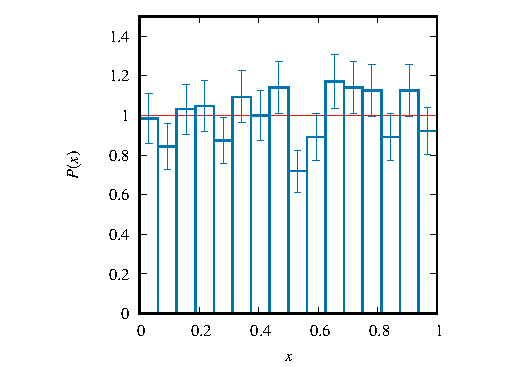
\includegraphics{image/histogram.pdf}}
\end{frame}

\begin{frame}[t,fragile]{ビンの個数の設定}
  \begin{itemize}
  \item 最適の幅というものはない
  \item 個数を増やすと表現の自由度は増えるが、各ビンのエラーバーが大きくなる
    \begin{itemize}
    \item データが統計的に独立である場合、それぞれのビンのカウント数$m$はポワソン分布に従う
    \item 統計誤差 $\sim \sqrt{m}$
    \end{itemize}
  \item いくつかの方法・公式が提案されているが、分布の形によっては不適切な場合も
    \begin{itemize}
    \item スタージェスの公式 $n = \log_2 N + 1$
    \item スコットの公式 $\Delta = 3.5 \sigma / N^{1/3}$
    \end{itemize}
  \item 実際には、ビンの個数を何通りか試してみるのが良い
  \item データを取り直すことが出来ない and/or コストがかかる場合も多いので、生データはいったんファイルに保存しておく
  \end{itemize}
\end{frame}

\end{document}

\section{モンテカルロ積分}

\begin{frame}[t,fragile]{モンテカルロ積分}
  \begin{itemize}
    \setlength{\itemsep}{1em}
  \item 円周率を与える公式
    \[
    \pi = \lim_{c \rightarrow \infty} \int_0^c f(x) \, dx \ \ \ f(x) = \frac{2}{\cosh x}
    \]
  \item スタンダードな数値積分法: 台形公式 (一次式補間), シンプソン公式 (二次式補間), etc
  \item カットオフ $c$ の値
    \begin{itemize}
    \item 誤差は $c$ が大きくなると指数関数的に小さくなる
    \item 例えば $c = 20$ で誤差は $8.3 \times 10^{-9}$ 以下
    \end{itemize}
  \end{itemize}
\end{frame}

\begin{frame}[t,fragile]{単純サンプリング}
  \begin{itemize}
    \setlength{\itemsep}{1em}
  \item $[0,c]$ と $[0,2]$ の一様分布から二次元上の点 $(x,y)$ を $M$ 組生成
  \item $f(x)$ の下に入った数 $N$ をカウント
    \[
    \pi \simeq 2c \times \frac{N}{M}
    \]
    \begin{tabular}{|c|c|c|}
      \hline
      $M$ & 平均値 & 誤差 \\
      \hline
      100 & 4.8 & 1.3 \\
      10000 & 3.12 & 0.11 \\
      1000000 & 3.154 & 0.011 \\
      \hline
    \end{tabular}
  \end{itemize}
  \vspace*{-7em}
  \hspace*{17em}
  \resizebox{!}{.45\textheight}{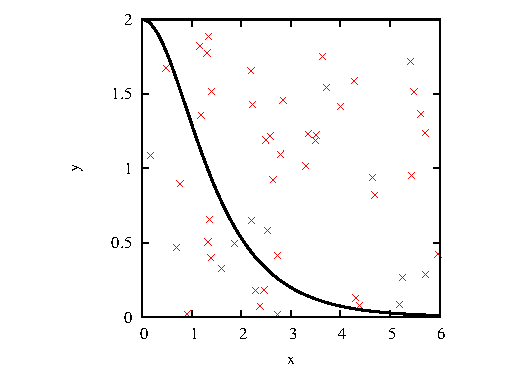
\includegraphics{image/coth-1.pdf}}
\end{frame}

\begin{frame}[t,fragile]{統計誤差の評価}
  \begin{itemize}
    \setlength{\itemsep}{1em}
  \item このモンテカルロ積分が実際に評価している積分
    \[
    \frac{1}{2c} \int_0^c \!\! \int_0^2 \!\! \theta(x,y) \, dx \, dy
    \ \ \ \theta(x,y) = \begin{cases} 2c & \text{if $y < f(x)$} \\ 0 & \text{otherwise} \end{cases}
    \]
  \item 統計誤差の評価
    \begin{itemize}
      \item 試行の成功確率(success probability): $q=\frac{\pi}{2c}$
      \item 一回の試行の平均値(mean): $\mu = 2c \times q = \pi$
      \item 分散(variance):
        \[ s^2 = (2c)^2q + 0^2(1-q) - \mu^2 = 2c\pi-\pi^2 = 4c^2 q(1-q) \]
      \item $c=20$ の時:
        \[ q \simeq 0.0785 \ \ \ s^2 \simeq 116
        \]
    \end{itemize}
  \end{itemize}
\end{frame}

\begin{frame}[t,fragile]{中心極限定理(central limiting theorem)}
  \begin{itemize}
    %\setlength{\itemsep}{1em}
  \item $M$回の試行のうち $N$回成功する確率 ($\pi$の見積もり値が $m=2cN/M$ となる確率)
    \[
    p(m=2c\frac{N}{M}) = \frac{M!}{N!(M-N)!} q^N (1-q)^{M-N}
    \]
  \item 両辺の対数をとってスターリングの公式を使う
    \[
    \log p(m) \simeq \frac{M}{2c} (m \log \frac{\pi}{m} + (2c-m)\log \frac{2c-\pi}{2c-m})
    \]
  \item $m$ に関して平均値 $\pi$ の周りで二次まで展開
    \[
    \log p(m) \simeq -\frac{M}{2s^2}(m-\pi)^2
    \]
  \item 分散$s^2/M$の正規分布(中心極限定理)
  \item 統計誤差は $\sqrt{M}$ に反比例して減少 $\Rightarrow$ 1桁小さくするには100倍の計算が必要
  \end{itemize}
\end{frame}

\begin{frame}[t,fragile]{単純サンプリング(2)}
  \begin{itemize}
    \setlength{\itemsep}{1em}
  \item $y$ に関してあらかじめ積分
  \item $[0,c]$の一様乱数 $x$ を用いて
    \[
    \int_0^c \frac{f(x)}{p(x)} p(x) \, dx \simeq \frac{1}{M} \sum_i c f(x_i) \ \ \ p(x) = \frac{1}{c}
    \]
    \begin{tabular}{|c|c|c|}
      \hline
      $M$ & 平均値 & 誤差 \\
      \hline
      100 & 3.1 & 0.8 \\
      10000 & 3.00 & 0.08 \\
      1000000 & 3.147 & 0.008 \\
      \hline
    \end{tabular}
  \end{itemize}
  \vspace*{-7em}
  \hspace*{17em}
  \resizebox{!}{.45\textheight}{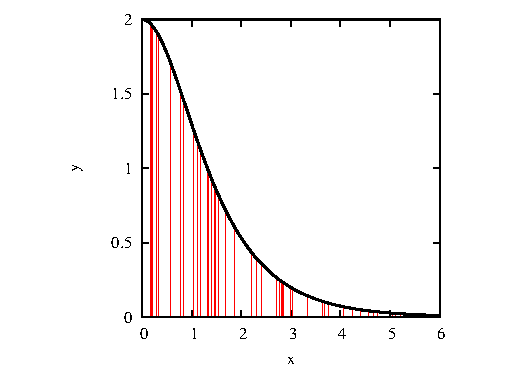
\includegraphics{image/coth-2.pdf}}
\end{frame}

\begin{frame}[t,fragile]{誤差の評価}
  \begin{itemize}
    \setlength{\itemsep}{1em}
  \item 関数 $f(x)/p(x)$ の分散
    \[
    s^2 = \int_0^c \Big(\frac{f(x)}{p(x)}\Big)^2 p(x) \, dx - \pi^2 = c \int_0^\infty f^2(x) \, dx - \pi^2 = 4c - \pi^2
    \]
  \item $c=20$ のとき $s^2 \simeq 70.1$
  \item 同じ試行回数 $M$ の時, 誤差は$\sqrt{70.1/116} = 0.77$ 倍
  \item もしくは $M$ を $116/70.1 = 1.65$ 倍したのと同じ効果
  \item 積分次元は低ければ低いほど良い
  \end{itemize}
\end{frame}

\begin{frame}[t,fragile]{次元の呪い(curse of dimensionality)}
  \begin{itemize}
    %\setlength{\itemsep}{1em}
  \item $n$次元超立方体(1辺の長さ 2, 体積 $2^n$)に対する$n$次元単位球の体積の割合
    \[
    q = \frac{\pi^{n/2} / \Gamma(\frac{n}{2}+1)}{2^n} \sim (\pi/n)^{n/2}
    \]
    $n=10$ で 0.2\%, $n=20$ で $10^{-8}$, $n=100$ で $10^{-70}$
  \item モンテカルロ積分で球の体積を計算しようとすると, 標準偏差に対する平均値の割合は指数関数的に小さい
    \[
    \frac{q}{\sqrt{q(1-q)}} \sim \sqrt{q}
    \]
  \item 次元が高くなるにつれて指数関数的に大きな $M$ が必要となる
  \item c.f. 通常の数値積分(台形公式等)でも同様
  \end{itemize}
\end{frame}

\begin{frame}[t,fragile]{重点的サンプリング}
  \begin{itemize}
    \setlength{\itemsep}{1em}
  \item (平均値が同じなら)被積分関数の分散が小さければ小さいほど良い (= 統計誤差が小さい)
  \item サンプリングの分布 $p(x)$ の形が $f(x)$ に近い程良い
  \item $f(x)$ の値が大きい所はより頻繁にサンプリング
  \item 重点的サンプリング (importance sampling)
  \end{itemize}
\end{frame}

\begin{frame}[t,fragile]{重点的サンプリング}
  \begin{itemize}
    \setlength{\itemsep}{1em}
  \item 積分への寄与が大きな箇所をより重点的にサンプリング
    \[
    p(x) = e^{-x}
    \]
    \begin{tabular}{|c|c|c|}
      \hline
      $M$ & 平均値 & 誤差 \\
      \hline
      100 & 3.06 & 0.06 \\
      10000 & 3.142 & 0.006 \\
      1000000 & 3.1412 & 0.0006 \\
      \hline
    \end{tabular}
  \end{itemize}
  \vspace*{-7em}
  \hspace*{17em}
  \resizebox{!}{.45\textheight}{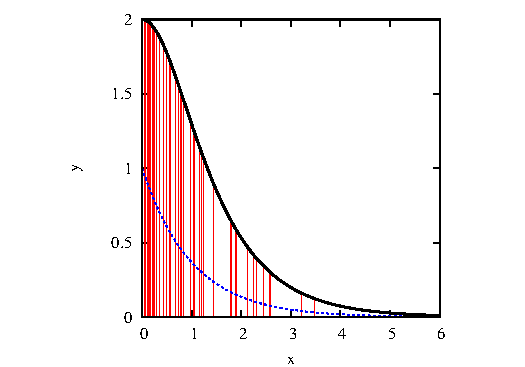
\includegraphics{image/coth-3.pdf}}
\end{frame}

\begin{frame}[t,fragile]{誤差のサンプル数依存性}
  \begin{itemize}
    \setlength{\itemsep}{1em}
  \item 関数 $f(x)/p(x)$ の分散
    \[
    s^2 = \int_0^c \Big(\frac{f(x)}{p(x)}\Big)^2 p(x) \, dx - \pi^2 \simeq 2(2+\pi) - \pi^2 = 0.414
    \]
  \item 同じ試行回数 $M$ の時, 誤差は

    $\sqrt{0.414/116} = 0.06 \mbox{倍}$

  \item もしくは $M$ を 280 倍したのと同じ
  \vspace*{-5em}
  \hspace*{15em}
  \resizebox{!}{.45\textheight}{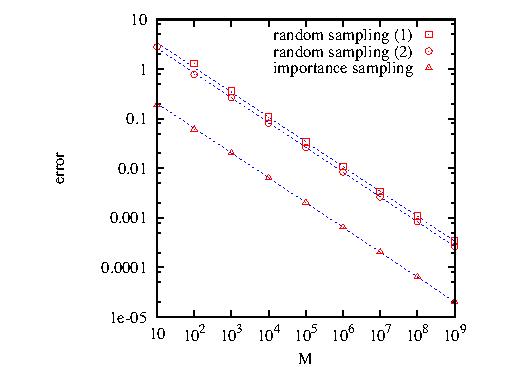
\includegraphics{image/sech-error.pdf}}
  \end{itemize}
\end{frame}

\begin{frame}[t,fragile]{理想的な重点的サンプリング?}
  \begin{itemize}
    \setlength{\itemsep}{1em}
  \item 理想的には $p(x)$ を $f(x)$ に比例するように取れば良い
  \item このとき $f(x) / p(x)$ は定数(分散 0) → 1回のサンプリングで厳密な結果が得られる???
  \item 実際には $p(x)$ が確率密度となるように規格化条件から定数 $c$ を決めておく必要あり
    \[
    \int p(x) \, dx = c \int f(x) \, dx = 1
    \]
  \item $c$ は今欲しい答そのもの!
  \end{itemize}
\end{frame}

%% % -*- coding: utf-8 -*-

\section{マルコフ連鎖モンテカルロ}

\begin{frame}[t,fragile]{統計物理における平衡状態}
  \begin{itemize}
    \setlength{\itemsep}{1em}
  \item Boltzmann分布 ($\beta \equiv 1/k_B T$)
    \[
    \pi(s) = \exp[-\beta {\cal H}(s)] \Big / \sum_s \exp[-\beta {\cal H}(s)]
    \]
  \item 物理量の期待値
    \[
    \langle A \rangle = \sum_s A(s) \exp[-\beta {\cal H}(s)] \Big/ \sum_s \exp[-\beta {\cal H}(s)]
    \]
  \item $\sum_s$は全ての状態に関する和 (系の体積に対して指数関数的に増加)
  \item 全ての状態について和をとるかわりに、Boltzmann重みが大きい(=$\cal H$が小さい)ところだけをモンテカルロ・サンプリング
  \end{itemize}
\end{frame}

%-*- coding:utf-8 -*-

\begin{frame}[t,fragile]{マルコフ連鎖モンテカルロ}
  \begin{itemize}
    %\setlength{\itemsep}{1em}
  \item 任意の多次元確率分布(今の場合はカノニカル分布)について、その分布したがうサンプル(状態)を生成する方法
    \begin{itemize}
    \item 直接カノニカル分布から独立したサンプリングをおこなうことは難しい
    \item 直前の状態からある確率にしたがって、次の状態を生成(マルコフ連鎖、Markov chain)
      \[
      \begin{split}
        &{\rm Pr}(X_{n+1}=s_j \,|\, X_0 = s_{i_0}, X_1 = s_{i_1}, \cdots, X_n = s_{i}) \\
        & \qquad = {\rm Pr}(X_{n+1}=s_j \,|\, X_n = s_{i}) = P_{i,j}
      \end{split}
      \]
    \item 長時間極限でカノニカル分布が達成されるように遷移確率(行列)$P_{i,j}$を選ぶ
      \[
      \lim_{n\rightarrow\infty}{\rm Pr}(X_n=s_j) \sim \pi_j = \exp[-\beta {\cal H}(s_j)]
      \]
    \end{itemize}
  \end{itemize}
\end{frame}

%-*- coding:utf-8 -*-

\begin{frame}[t,fragile]{遷移行列が満たすべき条件}
  \begin{itemize}
    % \setlength{\itemsep}{1em}
  \item 確率であるための条件: $0 \le P_{i,j} \le 1$
  \item 確率保存: $\sum_j P_{i,j} = 1$
  \item エルゴード性(ergodicity): \\
    ある整数$M$が存在し、$n \ge M$の全ての$n$で$(P^n)_{i,j} > 0$
  \item つりあいの条件(balance condition):
    \[ \sum_{i=1}^k \pi_i P_{i,j} = \pi_j \]
    カノニカル分布が固有値1の左固有ベクトル
  \end{itemize}
\end{frame}

\begin{frame}[t,fragile]{Perron-Frobeniusの定理}
  \begin{itemize}
    %\setlength{\itemsep}{1em}
  \item 正の正方行列$A$(すべての要素が正)について以下が成り立つ
    \begin{itemize}
      \item 他の全ての固有値よりも絶対値の大きな正の固有値$r$が存在する
      \item 固有値$r$は単純固有値である(縮退していない)
      \item 固有値$r$に対する右(左)固有ベクトル$v$ ($w$) は正のベクトルである
      \item 固有値 $r$ は $\displaystyle \min_i \sum_j a_{ij} \le r \le \max_i \sum_j a_{ij}$ を満たす
    \end{itemize}
  \item $A$が零の要素を持つ場合でも$A$が原始的(primitive = エルゴード的)である限り、上の結果は成り立つ
  \item 遷移行列は上の条件を満たす
    \begin{itemize}
    \item Boltzmann分布は絶対値最大の固有ベクトル
    \item 遷移行列を掛けていくとBoltzmann分布に収束
    \end{itemize}
  \end{itemize}
\end{frame}

\begin{frame}[t,fragile]{詳細つりあいの条件}
  \begin{itemize}
    \setlength{\itemsep}{1em}
  \item 実際には「つりあいの条件」よりもさらに厳しい「詳細つりあいの条件 (detailed balance condition)」を考えることが多い
    \[ \pi_i P_{i,j} = \pi_j P_{j,i} \]
  \item 両辺を $i$ について和をとると「つりあいの条件」に帰着する
  \item 「詳細つりあいの条件」は「つりあいの条件」の十分条件
  \end{itemize}
\end{frame}

%-*- coding:utf-8 -*-

\begin{frame}[t,fragile]{調和ポテンシャル中の古典粒子}
  \begin{itemize}
    %\setlength{\itemsep}{1em}
  \item ポテンシャルエネルギー
    \[ \hspace*{-4em} V(x) = x^2 \]
  \item カノニカル分布
    \[ \hspace*{-4em} P(x) = \frac{e^{-\beta V(x)}}{\int e^{-\beta V(x)} \, dx} \]
  \item 物理量の期待値
    \[ \hspace*{-4em} \langle x^2 \rangle = \frac{\int x^2 e^{-\beta V(x)} \, dx}{\int e^{-\beta V(x)} \, dx} \]
  \item 逆温度$\beta$が大きいと被積分関数の分散が非常に大きい $\Rightarrow$ 重点的サンプリング
  \end{itemize}
  \vspace*{-15em} \hfill
  \resizebox{4cm}{!}{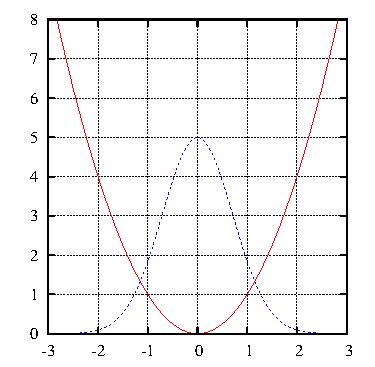
\includegraphics{image/harmonic.pdf}}
\end{frame}

%-*- coding:utf-8 -*-

\begin{frame}[t,fragile]{Metropolis法}
  \begin{itemize}
    %\setlength{\itemsep}{1em}
  \item 現在の配位$x$から、試行配位(trial configuration) $x'$を$x - \Delta \sim x + \Delta$の一様分布より選ぶ
  \item 確率$\min \Big( 1, \frac{e^{-\beta V(x')}}{e^{-\beta V(x)}} \Big)$で$x'$を採択(accept)。棄却(reject)された場合にはもとの$x$のまま
  \item 物理量の測定 (reject された場合にもカウントする)
  \item 採択確率(acceptance probability)は、$\frac{e^{-\beta V(x')}}{e^{-\beta V(x)}+e^{-\beta V(x')}}$でもよい
  \item 例: \href{https://github.com/todo-group/computer-experiments/blob/master/exercise/monte_carlo/harmonic.c}{harmonic.c}
  \end{itemize}
\end{frame}

\begin{frame}[t,fragile]{Metropolis法によるシミュレーション}
  \begin{itemize}
    \setlength{\itemsep}{1em}
  \item $\Delta = 0.1$
    
    \vspace*{-2em}\hfill \resizebox{9cm}{!}{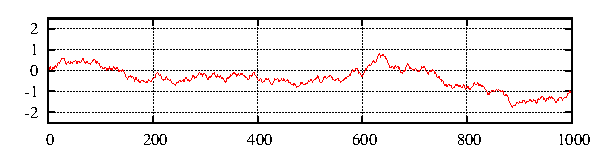
\includegraphics{image/series-001.pdf}}
  \item $\Delta = 1$
    
    \vspace*{-2em}\hfill \resizebox{9cm}{!}{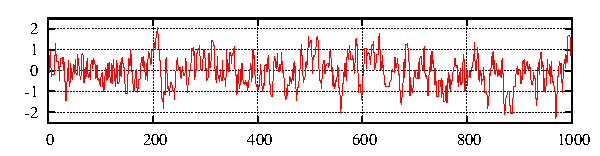
\includegraphics{image/series-010.pdf}}
  \item $\Delta = 10$
    
    \vspace*{-2em}\hfill \resizebox{9cm}{!}{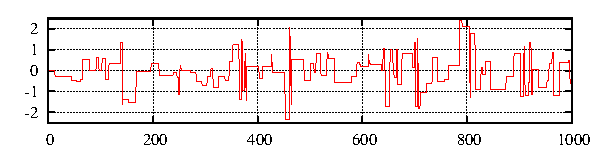
\includegraphics{image/series-100.pdf}}
  \end{itemize}
\end{frame}

%-*- coding:utf-8 -*-

\begin{frame}[t,fragile]{自己相関関数(autocorrelation function)}
  \begin{itemize}
    %\setlength{\itemsep}{1em}
  \item エルゴード性 + つりあい条件 ⇒ 原理的に正しいマルコフ連鎖モンテカルロ
  \item 実際には自己相関を考慮する必要あり
  \item 自己相関関数
    \[
    C(t) = \frac{\langle A_{i+t}A_i \rangle - \langle A \rangle^2}{\langle A^2 \rangle - \langle A \rangle^2} \sim \exp(-\frac{t}{\tau})
    \]
  \item $\tau$: 自己相関時間(autocorrelation time)
  \item 自己相関の影響により、統計的な「有効サンプル数」が減少
    \[
    M \rightarrow \frac{M}{1+2\tau}
    \]
  \end{itemize}
\end{frame}

\begin{frame}[t,fragile]{自己相関時間と統計誤差}
  \hspace*{4em} 自己相関時間 \hspace*{9em} 統計誤差

  \noindent\resizebox{0.49\textwidth}{!}{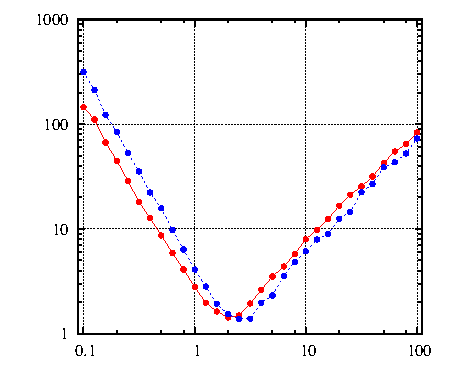
\includegraphics{image/autocorr.pdf}}
  \resizebox{0.49\textwidth}{!}{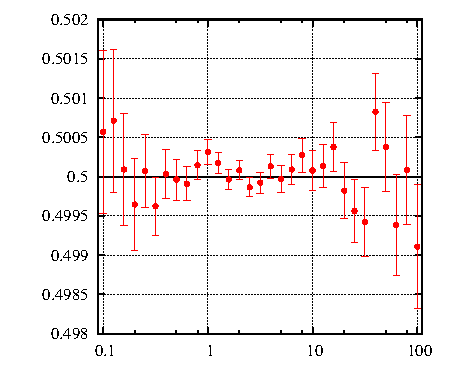
\includegraphics{image/error.pdf}}

  \hspace*{7em} $\Delta$ \hspace*{12em} $\Delta$
\end{frame}

\begin{frame}[t,fragile]{マルコフ連鎖モンテカルロ法}
  \begin{itemize}
    %\setlength{\itemsep}{1em}
  \item 統計誤差はサンプルの生の分散$s^2$とサンプル数$M$、自己相関時間$\tau$で決まる
    \[
    \sigma^2 \simeq \frac{s^2 (1+2\tau)}{M}
    \]
    \begin{itemize}
    \item 一度に大きく配位を動かそうとすると棄却率が増加 $\Rightarrow$ $\tau$が増加
    \item 動かす幅を小さくすると棄却率は高いが相関が消えない $\Rightarrow$ $\tau$が増加
    \item 非局所更新法、拡張アンサンブル法など様々な方法が使われている
    \end{itemize}
  \item 物理以外でも、Bayes推定や機械学習、社会現象のシミュレーションなど広く使われている
  \end{itemize}
\end{frame}

\begin{frame}[t,fragile]{イジング模型に対するモンテカルロ法}
  \begin{itemize}
    %\setlength{\itemsep}{1em}
  \item 更新の単位は一つのスピンとするのが一番自然
  \item メトロポリス法に必要なのは更新前後のエネルギー差だけなので、全エネルギーを計算しなおす必要なし
\begin{verbatim}
for (s = 0; s < num_sites; ++s) {
  delta = 0.0;
  for (j = 0; j < num_neighbors; ++j) {
    v = neighbor(s, j);
    delta += 2 * J * spin[s] * spin[v];
  }
  if (random() < exp(-beta * delta))
    spin[s] = -1 * spin[s];
}  
\end{verbatim}
  \end{itemize}
\end{frame}

\begin{frame}[t,fragile]{物理量の計算}
  \begin{itemize}
    %\setlength{\itemsep}{1em}
  \item 内部エネルギー$E$
    \begin{itemize}
    \item 初期状態のスピンを全て上向き(1)に取ると$E=-J \times \text{ボンド数}$
    \item モンテカルロステップ毎にエネルギーの変化分を計算しているので、採択された場合にはその値を足し込む
    \end{itemize}
  \item 比熱$C$: 内部エネルギーのゆらぎから計算できる
    \[
    C = \frac{1}{N} \frac{\partial E}{\partial T} = \frac{1}{NT^2} (\langle E^2 \rangle - \langle E \rangle^2)
    \]
  \item 磁化$m$: スピンの値の平均値 $m = \frac{1}{N} \sum_i \sigma_i$
    \begin{itemize}
    \item 外部磁場がない場合、対称性から$m$の長時間平均は厳密には零になる
    \item 熱力学極限では対称性が自発的に破れて、低温で有限の$m$
    \item シミュレーションでは$m$ではなく$m^2$を見るとよい
    \end{itemize}
  \end{itemize}
\end{frame}

%-*- coding:utf-8 -*-

\begin{frame}[t,fragile]{モンテカルロステップの設定}
  \begin{itemize}
    %\setlength{\itemsep}{1em}
  \item 全てのスピンについて一通り更新を試すのを、1モンテカルロステップと数える
  \item どれくらいのモンテカルロステップが必要かは、あらかじめは分からない
  \item 典型的には、$10^4$---$10^6$程度にとることが多い
  \item 熱平衡化 (thermalization)
    \begin{itemize}
    \item 初期配位依存性を取り除くため、モンテカルロステップの最初の部分は捨てる(burn-in time)
    \item 典型的には、全体の1割程度を捨てることが多い
    \end{itemize}
  \end{itemize}
\end{frame}



%% \section{二重井戸ポテンシャル}

\begin{frame}[t,fragile]{二重井戸ポテンシャル中の粒子}
  \begin{itemize}
    %\setlength{\itemsep}{1em}
  \item 時間依存しないシュレディンガー方程式
    \begin{align*}
      \big[ -\frac{d^2}{dx^2} + V(x) \big] \psi(x) = E \psi(x)
    \end{align*}
    ($\hbar^2/2m = 1$となるように単位をとった)
  \item 二重井戸ポテンシャル
    \begin{align*}
      V(x) = \begin{cases}
        \infty & \text{$x < 0$, $x > 1$} \\
        0 & \text{$0 < x < a$, $b < x < 1$} \\
        v & \text{$a < x < b$}
      \end{cases}
    \end{align*}
    ただし、$0<a<b<1$とする
  \item 境界条件: $\psi(0) = \psi(1) = 0$、$0 < x < 1$で$\psi(x)$とその導関数が連続
  \end{itemize}
\end{frame}

\begin{frame}[t,fragile]{シュレディンガー方程式の解法}
  \begin{itemize}
    % \setlength{\itemsep}{1em}
  \item シューティング
    \begin{itemize}
    \item 計算機実験I (L2)
    \item シューティングに用いる積分法: 2階常微分方程式の2次元1階連立微分方程式への書き換え、オイラー法とその改良、Numerov法
    \end{itemize}
  \item ハミルトニアンの対角化
    \begin{itemize}
    \item 計算機実験I (L4)
    \item 対角化手法: ハウスホルダー法(LAPACK)、べき乗法、Lanczos法
    \end{itemize}
  \item 変分法: 変分関数のパラメータの最適化
  \item その他の方法: 手で解けるところはあらかじめ解いて次元を減らす
  \item それぞれのコスト(=計算時間・メモリ)は?
  \end{itemize}
\end{frame}


%% \section{シューティング}

%% \begin{frame}[t,fragile]{準備: 微分方程式の書き換え}
  \begin{itemize}
    %\setlength{\itemsep}{1em}
  \item 2階の常微分方程式の一般形
    \[
    \frac{d^2y}{dx^2} + p(x)\frac{dy}{dx} + q(x)y = r(x)
    \]
  \item $y_1 \equiv y$, $y_2 \equiv \frac{dy}{dx}$とおくと
    \[
    \left\{
    \begin{array}{ccl}
      \frac{dy_1}{dx} & = & y_2 \\
      \frac{dy_2}{dx} & = & r(x) - p(x) y_2 - q(x) y_1
    \end{array}
    \right.
    \]
  \item さらに$\bm{y}\equiv(y_1, y_2)$, $\bm{f}(x, \bm{y})\equiv \left(y_2, r(x)-p(x)y_2 - q(x)y_1\right)$
    \[
    \frac{d\bm{y}}{dx} = \bm{f}(x, \bm{y})
    \]
  \item $n$階常微分方程式 $\Rightarrow$ $n$次元の1階常微分方程式
  \end{itemize}
\end{frame}

%% \begin{frame}[t,fragile]{初期値問題の解法 (Euler法)}
  \begin{itemize}
    %\setlength{\itemsep}{1em}
  \item $h$を微小量として微分を差分で近似する(前進差分)
    \[
    \frac{dy}{dt} \approx \frac{y(t+h) - y(t)}{h} = f(t, y)
    \]
  \item $t=0$における$y(t)$の初期値を$y_0$、$t_n \equiv nh$、$y_n$を$y(t_n)$の近似値とおくと、
    \[
    y_{n+1}-y_n = h f( t_n, y_n)
    \]
  \item Euler法
    \begin{itemize}
    \item $y_0$からはじめて、$y_1,y_2,\cdots$を順次求めていく
    \end{itemize}
  \end{itemize}
\end{frame}

%% \begin{frame}[t,fragile]{高次のRunge-Kutta法}
  \begin{itemize}
    %\setlength{\itemsep}{1em}
  \item 3次Runge-Kutta法
    \[
    \begin{array}{rcl}
      k_1 & = & h f(t_n, y_n) \\
      k_2 & = & h f(t_n + \frac{2}{3}h, y_n + \frac{2}{3}k_1) \\
      k_3 & = & h f(t_n + \frac{2}{3}h, y_n + \frac{2}{3}k_2) \\
      y_{n+1} & = & y_n + \frac{1}{4}k_1 + \frac{3}{8}k_2
      + \frac{3}{8}k_3
    \end{array}
    \]
  \item 4次Runge-Kutta法
    \[
    \begin{array}{rcl}
      k_1 & = & h f(t_n, y_n) \\
      k_2 & = & h f(t_n + \frac{1}{2}h, y_n + \frac{1}{2}k_1) \\
      k_3 & = & h f(t_n + \frac{1}{2}h, y_n + \frac{1}{2}k_2) \\
      k_4 & = & h f(t_n + h, y_n + k_3) \\
      y_{n+1} & = & y_n + \frac{1}{6}k_1 + \frac{1}{3}k_2
      + \frac{1}{3}k_3 + \frac{1}{6}k_4
    \end{array}
    \]
  \item 4次までは次数と$f$の計算回数が等しい
  \end{itemize}
\end{frame}

%% \begin{frame}[t,fragile]{計算コストと精度}
  \begin{itemize}
    %\setlength{\itemsep}{1em}
  \item 実際の計算では$f(t,y)$の計算にほとんどのコストがかかる
  \item 計算回数と計算精度の関係
    \begin{center}
      \begin{tabular}[h]{c|cccc}
        & 1次(Euler法) & 2次(中点法) & 3次 & 4次 \\
        \hline
        計算精度 & $O(h)$ & $O(h^2)$ & $O(h^3)$ & $O(h^4)$ \\
        計算回数 & $N$ & $2N$ & $3N$ & $4N$
      \end{tabular}
    \end{center}
  \item 高次のRunge-Kuttaを使う方が効率的
  \item どれくらい小さな$h$が必要となるか、前もっては分からない
  \item 刻み幅を変えて($h,h/2,h/4,\dots$)計算してみることが大事
    \begin{itemize}
    \item 誤差の評価
    \item 公式の間違いの発見
    \end{itemize}
  \end{itemize}
\end{frame}

%% \begin{frame}[t,fragile]{Numerov法}
  \begin{itemize}
    %\setlength{\itemsep}{1em}
  \item Numerov法
    \begin{itemize}
    \item 二階の常微分方程式で一階の項がない場合に使える
    \item 連立微分方程式に直さずに直接二階微分方程式を解く
    \item 4次の陰解法
    \item 方程式が線形の場合は陽解法に書き直せる
    \end{itemize}
  \item 微分方程式
    \[
    \frac{d^2y}{dx^2} = f(x,y)
    \]
  $y=y(x)$を$x=x_i$のまわりでテイラー展開する。$x_{i \pm 1} = x_i \pm h$での表式は
      \[
      y(x_{i \pm 1}) = y(x_i) \pm h y'(x_i) + \frac{h^2}{2} y''(x_i) \pm \frac{h^3}{6} y'''(x_i) + \frac{h^4}{24} y''''(x_i)  + O(h^5)
      \]
  \end{itemize}
\end{frame}

%% \begin{frame}[t,fragile]{Numerov法}
  \begin{itemize}
    \setlength{\itemsep}{1em}
  \item 二階微分の差分近似 ($y_i \equiv y(x_i)$等と書く)
    \[
    \frac{y_{i+1} - 2 y_i + y_{i-1}}{h^2} = y''_{i} + \frac{h^2}{12} y''''_{i} + O(h^4)
    \]
  一方で、微分方程式より
    \[
    y''''_i = \frac{d^2f}{dx^2}\Big|_{x=x_i} = \frac{f_{i+1}-2f_i+f_{i-1}}{h^2} + O(h^2)
    \]
    組み合わせると
    \[
    y_{i+1} = 2y_i - y_{i-1} + \frac{h^2}{12} (f_{i+1} + 10f_{i} + f_{i-1}) + O(h^6)
    \]
  \end{itemize}
\end{frame}

%% \begin{frame}[t,fragile]{Numerov法}
  \begin{itemize}
    %\setlength{\itemsep}{1em}
  \item 方程式が線形の場合、$f(x,y) = -a(x) y(x)$を代入すると
    \[
    y_{i+1} = 2y_i - y_{i-1} - \frac{h^2}{12} (a_{i+1}y_{i+1} + 10a_{i}y_{i} + a_{i-1}y_{i-1}) + O(h^6)
    \]
  $y_{i+1}$を左辺に集めると、陽解法となる
    \[
    y_{i+1} = \frac{2 (1-\frac{5h^2}{12} a_i)y_i - (1 + \frac{h^2}{12} a_{i-1}) y_{i-1}}{1 + \frac{h^2}{12} a_{i+1}} + O(h^6)
    \]
  \end{itemize}
\end{frame}

%% \begin{frame}[t,fragile]{ポアソン方程式の境界値問題}
  \begin{itemize}
    %\setlength{\itemsep}{1em}
  \item 二次元ポアソン方程式
    \[ \frac{\partial^2 u(x,y)}{\partial x^2} + \frac{\partial^2 u(x,y)}{\partial y^2} = f(x,y) \qquad 0 \le x \le 1, \ 0 \le y \le 1\]
  \item ディリクレ型境界条件: $u(x,y) = g(x,y)$ on $\partial \Omega$
  \item 有限差分法により離散化
    \begin{itemize}
    \item $x$方向、$y$方向をそれぞれ$n$等分: $(x_i,y_j) = (i/n, j/n)$
    \item $(n+1)^2$個の格子点の上で$u(x_i,y_j)=u_{ij}$が定義される
    \item そのうち$4n$個の値は境界条件で定まる
    \item ポアソン方程式を中心差分で近似 ($h=1/n$)
      \[
      \frac{u_{i+1,j}-2u_{ij}+u_{i-1,j}}{h^2} + \frac{u_{i,j+1}-2u_{ij}+u_{i,j-1}}{h^2} = f_{ij}
      \]
      残り$(n-1)^2$個の未知数に対する連立一次方程式
    \end{itemize}
  \end{itemize}
\end{frame}

%% \begin{frame}[t,fragile]{二分法}
  \begin{itemize}
    % \setlength{\itemsep}{1em}
  \item 反復法により一次元の方程式$f(x)=0$の解を求める
  \item 導関数を使わず関数値のみを利用 (c.f. ニュートン法)
  \item 初期条件として、$f(a) \times f(b) < 0$を満たす2点の組($a<b$)で解をはさみ込み、領域を狭めていく
  \item $a$と$b$の中点$x=(a+b)/2$を考える
    \begin{itemize}
    \item $|f(x)|$が十分小さい場合: $x$が解
    \item $f(a) \times f(x) < 0$の場合: $[a,x]$を新しい領域にとる
    \item $f(x) \times f(b) < 0$の場合: $[x,b]$を新しい領域にとる
    \end{itemize}
  \item 領域$[a,b]$の幅が十分小さくなったら終了
  \item 反復のたびに領域の幅は半分になる
  \item 全ての解を得られる保証はない
  \item 二分法の例: \href{https://github.com/todo-group/computer-experiments/blob/master/exercise/basics/bisection.c}{bisection.c}
  \end{itemize}
\end{frame}


%% \section{対角化による解法}

%% \begin{frame}[t,fragile]{対角化}
%%   \begin{itemize}
%%     \setlength{\itemsep}{1em}
%%   \item シュレディンガー方程式の行列表示
%%   \item ハウスホルダー法(LAPACK)
%%   \item べき乗法
%%   \item Lanczos法
%%   \item ハウスホルダー法によるプログラムの例: \href{https://github.com/todo-group/computer-experiments/blob/master/exercise/eigenvalue_problem/double_well.c}{double\_well.c}
%%   \end{itemize}
%% \end{frame}

%% \begin{frame}[t,fragile]{シュレディンガー方程式の行列表示}
  \begin{itemize}
    %\setlength{\itemsep}{1em}
  \item シュレディンガー方程式
    \[
    [-\frac{d^2}{dx^2}+V(x)]\psi(x) = E \psi(x)
    \]
  \item 連立差分方程式を行列の形で表す($\psi(x_0)=\psi(x_n)=0$)
    \begin{footnotesize}
    \[
    \begin{pmatrix}
      \frac{2}{h^2}+V(x_1) & -\frac{1}{h^2} \\
      -\frac{1}{h^2} & \frac{2}{h^2}+V(x_2) & -\frac{1}{h^2} \\
      & -\frac{1}{h^2} & \frac{2}{h^2}+V(x_3) & -\frac{1}{h^2} \\
      & & \ddots & \ddots \\
      & & & -\frac{1}{h^2} & \frac{2}{h^2}+V(x_{n-1}) \\
    \end{pmatrix}
    \begin{pmatrix}
      \psi(x_1) \\
      \psi(x_2) \\
      \psi(x_3) \\
      \vdots \\
      \psi(x_{n-1}) \\
    \end{pmatrix}
    = \cdots % E
    %% \begin{pmatrix}
    %%   \psi(x_1) \\
    %%   \psi(x_2) \\
    %%   \psi(x_3) \\
    %%   \vdots \\
    %%   \psi(x_{n-1}) \\
    %% \end{pmatrix}
    \]
    \end{footnotesize}
  \item $(n-1) \times (n-1)$の疎行列の固有値問題
    \begin{itemize}
    \item 固有値: 固有エネルギー
    \item 固有ベクトル: 波動関数
    \end{itemize}
  \end{itemize}
\end{frame}

%% \begin{frame}[t,fragile]{行列の数値対角化}
  \begin{itemize}
    %\setlength{\itemsep}{1em}
  \item 一般的に次元が5以上の行列の固有値は、あらかじめ定まる有限回の手続きでは求まらない
    \begin{itemize}
    \item 必ず何らかの反復法(+収束判定)が必要となる
    \end{itemize}
  \item 密行列向きの方法
    \begin{itemize}
    \item Jacobi法
    \item Givens変換・Householder法(三重対角化) + QR法など
    \end{itemize}
  \item 疎行列向きの方法
    \begin{itemize}
    \item べき乗法
    \item Lanczos法(三重対角化) + QR法など
    \end{itemize}
  \item 固有ベクトル
    \begin{itemize}
    \item QR法で求めたものを逆変換
    \item 逆反復法で精度改善
    \end{itemize}
  \end{itemize}
\end{frame}

%% \begin{frame}[t,fragile]{基本方針}
  \begin{itemize}
    %\setlength{\itemsep}{1em}
  \item やってはいけない方法: 特性方程式
    \[
    |\lambda E - A| = 0
    \]
    の係数を求めて、代数方程式として解く
    \begin{itemize}
    \item 数値的に不安定 (代数方程式の解は係数の誤差に対して敏感)
    \item 計算コスト大[$\sim O(N!)$]
    \end{itemize}
  \item スタンダードな方法: 行列を次々に直交変換して、対角行列(あるいは三重対角行列)に近づけていく
    \[
    A \rightarrow U_1^T A U_1 \rightarrow U_2^T (U_1^T A U_1) U_2 \rightarrow U_3^T (U_2^T (U_1^T A U_1) U_2) U_3 \rightarrow \cdots
    \]
  \item 固有値は変換された行列の固有値、固有ベクトルは変換後の行列の固有ベクトルに左から$U_1 U_2 U_3 \cdots$を掛けたもの
  \end{itemize}
\end{frame}

%% \begin{frame}[t,fragile]{LAPACKの対角化ルーチン}
  \begin{itemize}
    %\setlength{\itemsep}{1em}
  \item 様々な対角化ルーチンが準備されている
    \begin{itemize}
    \item 倍精度実対称行列の対角化 {\tt dsyev}
      \url{http://www.netlib.org/lapack/explore-html/dd/d4c/dsyev_8f.html}
    \item Fortranによる関数宣言
\begin{lstlisting}
subroutine dsyev(character JOBZ, character UPLO,
  integer N, double precision, dimension(lda, *) A,
  integer LDA, double precision, dimension(*) W,
  double precision, dimension(*) WORK,
  integer LWORK, integer INFO)		
\end{lstlisting}
    \end{itemize}
  \item 他にも{\tt dsyevd}、{\tt dsyevr}、{\tt dsyevx}などがある \\
    3重対角化までは同じ。3重対角行列の対角化が異なる
  \item 単精度版の{\tt ssyev}、複素(エルミート行列)版の{\tt zheev}など
  \item {\tt dsyev}の使用例: \href{https://github.com/todo-group/computer-experiments/blob/master/exercise/eigenvalue_problem/diag.c}{diag.c}
  \end{itemize}
\end{frame}

%% %\begin{frame}[t,fragile]{CからBLAS/LAPACKを呼び出す際の注意事項}
  \begin{itemize}
    %\setlength{\itemsep}{1em}
  \item (もともとFortran言語で書かれていたことによる制限)
  \item 関数名はすべて小文字、最後に \verb+_+ (下線)を付ける
  \item スカラー、ベクトル、行列は全て「ポインタ渡し」とする
  \item ベクトルや行列は最初の要素へのポインタを渡す (サイズは別に渡す)
  \item 行列の要素は(0,0) $\rightarrow$ (1,0) $\rightarrow$ (2,0) $\rightarrow\cdots\rightarrow$ $(m-1,0)$ $\rightarrow$ (0,1) $\rightarrow$ (1,1) $\rightarrow\cdots\rightarrow$ $(m-1,n-1)$の順で連続して並んでいなければならない(column-major)
    \begin{itemize}
    \item C言語の二次元配列では \verb+a[i][j]+ の次には \verb%a[i][j+1]%が入っている(row-major)
    \item 行列が転置されて解釈されてしまう!
    \end{itemize}
  \item コンパイル時には{\tt -llapack -lblas}オプションを指定し、LAPACKライブラリとBLASライブラリをリンクする(ハンドブック2.1.6節)
  \end{itemize}
\end{frame}

%% \begin{frame}[t,fragile]{cmatrix.hライブラリ}
  \begin{itemize}
    %\setlength{\itemsep}{1em}
  \item Column-major形式の二次元配列の確保({\tt alloc\_dmatrix})、開放({\tt free\_dmatrix})、出力({\tt print\_dmatrix})、読み込み({\tt read\_dmatrix})を行うためのユーティリティ関数、(i,j)成分にアクセスするためのマクロ({\tt mat\_elem})他を準備
  \item ソースコード: \href{https://github.com/todo-group/computer-experiments/blob/master/exercise/matrix/cmatrix.h}{cmatrix.h}
  \item 使用例
\begin{lstlisting}
#include "cmatrix.h"
...
double **mat;
mat = alloc_dmatrix(m, n);
mat_elem(mat, 1, 3) = 5.0;
...
free_dmatrix(mat);
\end{lstlisting}
  \item サンプルコード: \href{https://github.com/todo-group/computer-experiments/blob/master/exercise/matrix/matrix_example.c}{matrix\_example.c}
  \end{itemize}
\end{frame}

%% %\begin{frame}[t,fragile]{alloc\_dmatrixでの動的二次元配列の確保}
  \begin{itemize}
    %\setlength{\itemsep}{1em}
  \item 長さ$m \times n$の一次元配列を用意し、各列(それぞれ$m$要素)の先頭アドレスを長さ$n$のポインター配列に格納する (ハンドブック2.12.3節)
\begin{lstlisting}
double **a;
m = 10;  
n = 10;  
a = (double**)malloc((size_t)(n * sizeof(double*));
a[0] = (double*)malloc((size_t)(m*n * sizeof(double));
for (int i = 1; i < n; ++i)
  a[i] = a[i-1] + m;
\end{lstlisting}
\item 行列の(i,j)成分を\verb+a[j][i]+に格納することにする (column-major)
  \end{itemize}
\end{frame}

%% \begin{frame}[t,fragile]{要素アクセス・先頭アドレス}
  \begin{itemize}
    % \setlength{\itemsep}{1em}
  \item 行列の(i,j)成分は\verb+a[j][i]+に格納されている
    \begin{itemize}
      \item \href{https://github.com/todo-group/computer-experiments/blob/master/exercise/matrix/cmatrix.h}{cmatrix.h}ではマクロ(\verb+mat_elem+)を準備
\begin{lstlisting}
#define mat_elem(mat, i, j) (mat)[j][i]
\end{lstlisting}
\item このマクロを使うと、例えば(i,j)成分への代入は以下のように書ける
\begin{lstlisting}
mat_elem(a, i, j) = 1;
\end{lstlisting}
\end{itemize}
  \item LAPACKにベクトルや行列の最初の要素へのポインタを渡す
    \begin{itemize}
      \item ベクトルの最初の要素(0)へのポインタ: \verb+&v[0]+
      \item 行列の最初の要素(0,0)へのポインタ: \verb+&a[0][0]+
      \item \href{https://github.com/todo-group/computer-experiments/blob/master/exercise/matrix/cmatrix.h}{cmatrix.h}にマクロ({\tt vec\_ptr}、{\tt mat\_ptr})が準備されているのでそれぞれ、{\tt vec\_ptr(v)}、{\tt mat\_ptr(a)}と書ける
    \end{itemize}
  \end{itemize}
\end{frame}

%% \begin{frame}[t,fragile]{反復法}
  \begin{itemize}
    %\setlength{\itemsep}{1em}
  \item 疎行列の場合、行列ベクトル積は高速に行える
  \item Givens変換、Householder変換などを行うと疎行列性が失われる
  \item 行列ベクトル積のみを用いる反復法が効果的
    \begin{itemize}
    \item べき乗法
    \item Lanczos法
    \end{itemize}
  \end{itemize}
\end{frame}

%% \begin{frame}[t,fragile]{べき乗法(Power Method)}
  \begin{itemize}
    %\setlength{\itemsep}{1em}
  \item 適当なベクトル$v_1$から出発する
  \item $v_1$が最大固有ベクトル$\xi_1$と直交していないとすると
    \[
    v_1 = c_1 \xi_1 + c_2 \xi_2 + c_3 \xi_3 + \cdots + c_N \xi_N
    \]
    と展開できる($c_1 \ne 0$)。この両辺に$A$を次々掛けて行くと
    \begin{align*}
      v_2 = A v_1 &= c_1 \lambda_1 \xi_1 + c_2 \lambda_2 \xi_2 + c_3 \lambda_3 \xi_3 + \cdots + c_N \lambda_N \xi_N \\
      v_3 = A^2 v_1 &= c_1 \lambda_1^2 \xi_1 + c_2 \lambda_2^2 \xi_2 + c_3 \lambda_3^2 \xi_3 + \cdots + c_N \lambda_N^2 \xi_N \\
      \vdots \\
      v_{n+1} = A^n v_1 &= c_1 \lambda_1^n \xi_1 + c_2 \lambda_2^n \xi_2 + c_3 \lambda_3^n \xi_3 + \cdots + c_N \lambda_N^n \xi_N \\
      &= c_1 \lambda_1^n \Big[ \xi_1 + \sum_{k=2}^N \frac{c_k}{c_1} \big( \frac{\lambda_k}{\lambda_1}\big)^n \xi_k \Big] \approx c_1 \lambda_1^n \xi_1 \\
    \end{align*}
  \end{itemize}
\end{frame}

%% \begin{frame}[t,fragile]{べき乗法の収束}
  \begin{itemize}
    %\setlength{\itemsep}{1em}
  \item べき乗法による固有値
    \[
    \frac{v_{k+1}^T v_{k+1}}{v_{k+1}^T v_k} = \lambda_1 + O\Big( \big(\frac{\lambda_2}{\lambda_1} \big)^{2k}\Big)
    \]
  \item 誤差の収束
    \[
    \frac{v_{k+1}^T v_{k+1}}{v_{k+1}^T v_k} \approx \lambda_1 + e^{-2k \ln (\lambda_1/\lambda_2)}
    \]
  \item $1 / \ln (\lambda_1/\lambda_2)$ 程度の反復が必要
  \item $\lambda_1$と$\lambda_2$が近い場合には、反復回数が非常に多くなる
  \end{itemize}
\end{frame}

%% \begin{frame}[t,fragile]{Rayleigh-Ritzの方法}
  \begin{itemize}
    \setlength{\itemsep}{1em}
  \item $N \times N$行列$A$について、互いに正規直交するベクトル$v_1,v_2,\cdots,v_M$ ($M < N$)が張る部分空間の中で「最良の」固有ベクトルを求めたい
  \item $N \times M$行列
    \[
    V=(v_1 v_2 \cdots v_M)
    \]
    を定義すると、$V^TV=I$が成り立つ(ただし$VV^T \ne I$)
  \item 部分空間内のベクトルを$w = \sum_i a_i v_i$と表すと、$\frac{w^TAw}{w^Tw}$が極大値を取る(本当の固有ベクトルにできるだけ平行になる)条件は、
    \[
    \frac{\partial}{\partial a_i} \frac{w^TAw}{w^Tw} \sim \sum_j H_{ij}a_j - \lambda a_i = 0
    \]
  \end{itemize}
\end{frame}

%% \begin{frame}[t,fragile]{Rayleigh-Ritzの方法}
  \begin{itemize}
    %\setlength{\itemsep}{1em}
  \item $m \times m$行列
    \[
    H = V^T A V
    \]
    に対する固有値問題 $H a = \lambda a$
  \item $\lambda$: もとの行列の近似固有値(Ritz値)
  \item $Va$: もとの行列の近似固有ベクトル(Ritzベクトル)
  \item 最大固有値に対する近似固有値が欲しい場合、最大固有ベクトルになるべく近い(しかし互いに直交する)ベクトル$v_1,v_2,\cdots,v_m$を選べばよい
  \end{itemize}
\end{frame}

%% \begin{frame}[t,fragile]{Lanczos法}
  \begin{itemize}
    \setlength{\itemsep}{1em}
  \item 初期(ランダム)ベクトル$v_1$に加えて
    \[
    Av_1, Av_1, \cdots A^{m-1}v_1
    \]
    を正規直交化して$v_1,v_2,\cdots,v_m$を作る(Krylov部分空間)
  \item 部分空間でのRitz値を固有値の近似値とする
  \item $A^kv_1$はどんどん最大固有ベクトルに近づいていくので、$m \ll n$でも良い近似固有値が得られると期待される
  \end{itemize}
\end{frame}


%% %-*- coding:utf-8 -*-

\section{変分法}

%-*- coding:utf-8 -*-

\begin{frame}[t,fragile]{変分法}
  \begin{itemize}
    %\setlength{\itemsep}{1em}
  \item 波動関数を互いに直交する正規化された波動関数(基底関数)の線形結合で近似する (変分波動関数、試行関数)
    \begin{align*}
      | \psi \rangle = \sum_{p=1}^m C_p | \phi_p \rangle \qquad (\langle \phi_p | \phi_q \rangle = \delta_{pq})
    \end{align*}
  \item エネルギーの期待値
    \begin{align*}
      E &= \frac{\langle \psi | H | \psi \rangle}{\langle \psi | \psi \rangle} = \frac{\sum_{p,q} C_p^* H_{pq} C_q}{\sum_{p,q} C_p^* \delta_{pq} C_q} \\
      H_{pq} &= \langle \phi_p | H | \phi_q \rangle
    \end{align*}
  \item $E$ができるだけ小さくなるよう係数$C_p$を最適化 (変分原理)
  \end{itemize}
\end{frame}

%-*- coding:utf-8 -*-

\begin{frame}[t,fragile]{変分法}
  \begin{itemize}
    %\setlength{\itemsep}{1em}
  \item $\delta E = 0$から
    \begin{align*}
      \sum_{q} (H_{pq} - E \delta_{pq} ) C_q = 0 \qquad \text{for $^\forall p$}
    \end{align*}
  \item $H_{pq}$, $\delta_{pq}$を$m \times m$行列と考えると、固有値問題とみなせる
    \begin{align*}
      H C = E C
    \end{align*}
  \item $H$はエルミート行列
  \item $\{ \phi_p \}$の張る部分空間での最適化 (= Rayleigh-Ritzの方法)
  \item 変分波動関数と真の波動関数の差が$\epsilon$程度の時、$E$と真の固有エネルギーの差は$\epsilon^2$程度
  \end{itemize}
\end{frame}

%-*- coding:utf-8 -*-

\begin{frame}[t,fragile]{非直交基底関数による変分法}
  \begin{itemize}
    %\setlength{\itemsep}{1em}
  \item 重なり積分
    \begin{align*}
      S_{pq} = \langle \phi_p | \phi_q \rangle \ne \delta_{pq}
    \end{align*}
  \item 変分波動関数の正規化条件
    \begin{align*}
      \langle \psi | \psi \rangle = \sum_{p,q} C_p^* \langle \phi_p | \phi_q \rangle C_q = \sum_{p,q} C_p^* S_{pq} C_q = 1
    \end{align*}
  \item エネルギー期待値
    \begin{align*}
      E = \frac{\sum_{p,q} C_p^* H_{pq} C_q}{\sum_{p,q} C_p^* S_{pq} C_q}
    \end{align*}
  \item $\delta E = 0$から
    \begin{align*}
      \sum_q (H_{pq} - E S_{pq}) C_q = 0 \ \Rightarrow \ HC = ESC \ \text{(一般化固有値問題)}
    \end{align*}
  \end{itemize}
\end{frame}

%-*- coding:utf-8 -*-

\begin{frame}[t,fragile]{一般化固有値問題}
  \begin{itemize}
    %\setlength{\itemsep}{1em}
  \item 重なり行列 $S_{pq} = \langle \phi_p | \phi_q \rangle$
    \begin{itemize}
      \item エルミート行列: $S_{pq} = S_{qp}^*$
      \item 正定値 ($\{\phi_p\}$が線形独立の場合):
        \begin{align*}
          x^\dagger S x = \sum_{pq} \langle \phi_p | \phi_q \rangle x_p^* x_q = || \sum_p x_p | \phi_p \rangle ||^2 > 0
        \end{align*}
    \end{itemize}
  \item 一般化固有値問題 $\Rightarrow$ 2回の固有値分解により解くことができる
    \begin{itemize}
      \item $S$を固有値分解: $S = U D U^\dagger$
      \item $S$固有値は全て正 $\Rightarrow$ $D^{-1/2}$を定義可
      \item $HC=ESC$ $\Rightarrow$ $D^{-1/2} U^\dagger H U D^{-1/2} D^{1/2} U^\dagger C = E D^{1/2} U^\dagger C$
      \item $H' = D^{-1/2} U^\dagger H U D^{-1/2}$、$C'D^{1/2} U^\dagger C$とおくと
        \begin{align*}
          H'C' = EC' \qquad \text{(通常の)固有値問題}
        \end{align*}
      \item (1回目の固有値分解はコレスキー分解$A=L L^\dagger$ ($L$は下三角行列)を用いてもよい)
    \end{itemize}
  \end{itemize}
\end{frame}



%% \section{解析計算による次元削減}

\begin{frame}[t,fragile]{シュレディンガー方程式の一般解}
  \begin{itemize}
    %\setlength{\itemsep}{1em}
  \item 二重井戸ポテンシャル
    \begin{align*}
      V(x) = \begin{cases}
        \infty & \text{$x < 0$, $x > 1$} \\
        0 & \text{$0 < x < a$, $b < x < 1$} \\
        v & \text{$a < x < b$}
      \end{cases}
    \end{align*}
  \item それぞれの領域内では手で解ける
  \item 領域1 ($0 < x < a$)、領域3 ($b < x < 1$)では
    \begin{align*}
      -\frac{d^2}{dx^2}\psi(x) = E\psi(x)
    \end{align*}
  \end{itemize}
\end{frame}

\begin{frame}[t,fragile]{シュレディンガー方程式の一般解}
  \begin{itemize}
    %\setlength{\itemsep}{1em}
  \item 領域1 ($0 < x < a$)、領域3 ($b < x < 1$)における一般解
    \begin{align*}
      \psi(x) &= A_1 e^{i\sqrt{E}x} + B_1 e^{-i\sqrt{E}x} \\
      \psi(x) &= A_3 e^{i\sqrt{E}x} + B_3 e^{-i\sqrt{E}x}
    \end{align*}
    あきらかに$E>0$であるので
    \begin{align*}
      \psi(x) &= \alpha_1 \cos(\sqrt{E}x) + \beta_1 \sin(\sqrt{E}x) \\
      \psi(x) &= \alpha_3 \cos(\sqrt{E}x) + \beta_3 \sin(\sqrt{E}x)
    \end{align*}
  \end{itemize}
\end{frame}

\begin{frame}[t,fragile]{シュレディンガー方程式の一般解}
  \begin{itemize}
    %\setlength{\itemsep}{1em}
  \item 領域2 ($a < x < b$)における一般解
    \begin{align*}
      \psi(x) &= A_2 e^{i\sqrt{(E-v)}\,x} + B_1 e^{-i\sqrt{(E-v)}\,x}
    \end{align*}
  \item $E < v$の場合
    \begin{align*}
      \psi(x) &= \alpha_2 \exp(-\sqrt{(v-E)}\,x) + \beta_2 \exp(\sqrt{(v-E)}\,x)
    \end{align*}
  \item $E > v$の場合
    \begin{align*}
      \psi(x) &= \alpha_2 \cos(\sqrt{(E-v)}\,x) + \beta_2 \sin(\sqrt{(E-v)}\,x)
    \end{align*}
  \end{itemize}
\end{frame}

\begin{frame}[t,fragile]{シュレディンガー方程式の一般解}
  \begin{itemize}
    %\setlength{\itemsep}{1em}
  \item 境界条件($E < v$の場合)
    \begin{align*}
      &\alpha_1 = 0 \\
      &\alpha_1 \cos(\sqrt{E}a) + \beta_1 \sin(\sqrt{E}a) \\
      & \qquad =
      \alpha_2 \exp(-\sqrt{(v-E)}\,a) + \beta_2 \exp(\sqrt{(v-E)}\,a) \\
      &-\alpha_1 \sqrt{E} \sin(\sqrt{E}a) + \beta_1 \sqrt{E} \sin(\sqrt{E}a) \\
      & \qquad =
      - \alpha_2 \sqrt{(v-E)} \exp(-\sqrt{(v-E)}\,a) + \beta_2 \sqrt{(v-E)} \exp(\sqrt{(v-E)}\,a) \\
      &\cdots
    \end{align*}
  \item $\beta_1$, $\alpha_2$, $\beta_2$, $\alpha_3$, $\beta_3$ に関する連立方程式: $M x = 0$
  \item $5 \times 5$行列$M$は$E$の(非線形な)関数
  \item 非自明な解が存在するための条件: $\det M=0$
  \end{itemize}
\end{frame}


%% \begin{frame}[t,fragile]{行列式の計算}
%%   \begin{itemize}
%%     \setlength{\itemsep}{1em}
%%   \item ガウスの消去法とLU分解
%%   \item LU分解による行列式の計算
%%   \item LAPACKによるLU分解
%%   \item LU分解のプログラムの例: \href{https://github.com/todo-group/computer-experiments/blob/master/exercise/linear_system/lu_decomp.c}{lu\_decomp.c}
%%   \item 行列式計算のプログラムの例: \href{https://github.com/todo-group/computer-experiments/blob/master/exercise/linear_system/determinant.c}{determinant.c}
%%   \end{itemize}
%% \end{frame}

%% \begin{frame}[t,fragile]{逆行列の「間違った」求め方}
  \begin{itemize}
    \setlength{\itemsep}{1em}
  \item 線形代数の教科書に載っている公式
    \[
    A^{-1} = \frac{\tilde{A}}{|A|}
    \]
    $|A|$: $A$の行列式、$\tilde{A}$: $A$の余因子行列
  \item $n \times n$行列の行列式を定義通り計算すると、計算量〜$O(n!)$
  \item したがって、上の方法で逆行列を計算すると、計算量〜$O(n!)$
  \item $n=100$の場合: $n! \approx 9.3 \times 10^{157}$
  \end{itemize}
\end{frame}

%% \begin{frame}[t,fragile]{逆行列の「正しい」求め方}
  \begin{itemize}
    \setlength{\itemsep}{1em}
  \item 連立一次方程式 $A {\bf x} = {\bf e}_j$ を全ての${\bf e}_j$について解く
  \item Gaussの消去法による連立一次方程式の解法: 計算量〜$O(n^3)$
  \item Gaussの消去法の途中で出てくる下三角行列(L)と上三角行列(U)行列を再利用(LU分解)すれば、逆行列全体を求めるための計算量も$O(n^3)$
  \item 行列式も$O(n^3)$で計算可
  \item $n=100$の場合: $n^3 = 10^6 \ll 9.3 \times 10^{157}$
  \end{itemize}
\end{frame}

%% \begin{frame}[t,fragile]{LU分解}
  \begin{itemize}
    %\setlength{\itemsep}{1em}
  \item LU分解による連立一次方程式の解法
    \begin{itemize}
    \item 方程式は$A{\bf x} = LU{\bf x} = {\bf b}$と書ける
    \item まず、$L{\bf y} = {\bf b}$を解いて、${\bf y}$を求める(前進代入)
    \item 次に、$U{\bf x} = {\bf y}$を解いて、${\bf x}$を求める(後退代入)
    \end{itemize}
  \item 計算量はガウスの消去法と変わらない
  \item 一度LU分解をしておけば、異なる${\bf b}$に対する解も簡単に求められる \\[2em]
  \item 行列式は$U$の対角成分の積で与えられる (ピボット選択する場合は、行の入れ替えにより符号が変わることに注意)
  \end{itemize}
\end{frame}


%% \begin{frame}[t,fragile]{LAPACKによる連立一次方程式の求解}
  \begin{itemize}
    \setlength{\itemsep}{1em}
  \item LU分解を行うサブルーチン {\tt dgetrf} \\
    \url{http://www.netlib.org/lapack/explore-html/d3/d6a/dgetrf_8f.html}
  \item Fortranによる関数宣言
\begin{lstlisting}
subroutine dgetrf(integer M, integer N,
         double precision, dimension(lda, *) A,
         integer LDA, integer, dimension(*) IPIV,
         integer INFO)
\end{lstlisting}
\item {\tt A}: 左辺の行列、{\tt M,N}: 次元、{\tt IPIV}: 選択されたピボット行のリスト、{\tt lda}: 通常{\tt M} (行数)と同じで良い
  \end{itemize}
\end{frame}

%% \begin{frame}[t,fragile]{LAPACKによる連立一次方程式の求解}
  \begin{itemize}
    \setlength{\itemsep}{1em}
  \item C言語から呼び出すための関数宣言を作成 (ハンドブック2.7.4節)
\begin{lstlisting}
void dgetrf_(int *M, int *N, double *A,
             int *LDA, int*IPIV, int *INFO);
\end{lstlisting}
関数名は全て小文字。関数名の最後に {\tt \_} (下線)を付ける
\item LU分解の例
\begin{lstlisting}
m = 10;
n = 10;
a = alloc_dmatrix(m, n);
...
dgetrf_(&m, &n, mat_ptr(a), &m, vec_ptr(ipiv), &info);
\end{lstlisting}
完全なソースコード: \href{https://github.com/todo-group/computer-experiments/blob/master/exercise/linear_system/lu_decomp.c}{lu\_decomp.c}
  \end{itemize}
\end{frame}


%% \begin{frame}[t,fragile]{まとめ}
%%   \begin{itemize}
%%     \setlength{\itemsep}{1em}
%%   \item 一次元(一粒子)シュレディンガー方程式の固有値問題
%%     \begin{itemize}
%%     \item シューティングによる方法: 連立微分方程式の積分、二分法
%%     \item 対角化による方法: 差分化、ハウスホルダー法、べき乗法、Lanczos法
%%     \item 変分法(線形の場合): 固有値問題、一般化固有値問題
%%     \item 特別な場合に有効な方法: LU分解
%%     \end{itemize}
%%   \item 計算精度は何で決まるか?
%%   \item それぞれのコスト(=計算時間・メモリ)は?
%%   \end{itemize}
%% \end{frame}

\end{document}
